\documentclass[../../../main]{subfiles}
\begin{document}

\section{結果}

\subsection{実験1}
アモルファス太陽電池とシリコンフォトダイオードのそれぞれに、実験室の照明(蛍光灯)下・蓋をして光を遮った状態(暗時)・LEDライトを直接照射したとき・MAGライトを直接照射ときの4パターンで電流と電圧の変化を測定した。
測定した最大の電流と電圧の結果を表\ref{tab:exp1}に示す。
%Please add the following packages if necessary:
%\usepackage{booktabs, multirow} % for borders and merged ranges
%\usepackage{soul}% for underlines
%\usepackage[table]{xcolor} % for cell colors
%\usepackage{changepage,threeparttable} % for wide tables
%If the table is too wide, replace \begin{table}[!htp]...\end{table} with
%\begin{adjustwidth}{-2.5 cm}{-2.5 cm}\centering\begin{threeparttable}[!htb]...\end{threeparttable}\end{adjustwidth}
\begin{table}[!htp]\centering
	\caption{さまざまな光源下での電流・電圧}\label{tab:exp1}
	\scriptsize
	\begin{tabular}{ccccc}\toprule
		       & \multicolumn{2}{c}{太陽電池} & \multicolumn{2}{c}{フォトダイオード}                     \\\cmidrule{2-5}
		       & A                        & V                            & A       & V       \\\midrule
		蛍光灯下   & 0.00017                  & 2.7621                       & 0.00002 & 0.30601 \\
		暗時     & 0.00003                  & 1.9265                       & 0.00001 & 0.23010 \\
		LEDライト & 0.00127                  & 3.2019                       & 0.00037 & 0.46318 \\
		MAGライト & 0.00038                  & 2.9753                       & 0.00769 & 0.58717 \\
		\bottomrule
	\end{tabular}
\end{table}


\subsection{実験2}\label{subsec:exp2}
Variable Power Supply(以後VPS)を用いて\SI{0}{A}から、\SI{12}{A}間の設定電流に対してその出力をDegital Multimeter(以後DMM)で測定した。
その結果を表\ref{tab:exp2}に示す。
また、これを元にグラフにすると図\ref{fig:exp2}のようになる。
%Please add the following packages if necessary:
%\usepackage{booktabs, multirow} % for borders and merged ranges
%\usepackage{soul}% for underlines
%\usepackage[table]{xcolor} % for cell colors
%\usepackage{changepage,threeparttable} % for wide tables
%If the table is too wide, replace \begin{table}[!htp]...\end{table} with
%\begin{adjustwidth}{-2.5 cm}{-2.5 cm}\centering\begin{threeparttable}[!htb]...\end{threeparttable}\end{adjustwidth}

\begin{table}[!htp]\centering
	\caption{VPSの設定電流とDMMでの計測値}\label{tab:exp2}
	\scriptsize
	\begin{tabular}{cc}\toprule
		VPS上の設定電流 / \si{A} & DMMでの計測値 / \si{A} \\\midrule
		0                  & 0.3355            \\
		0.2                & 0.33294           \\
		0.4                & 0.39245           \\
		0.5                & 0.48868           \\
		0.6                & 0.58391           \\
		0.7                & 0.69338           \\
		0.8                & 0.78972           \\
		0.9                & 0.88524           \\
		1.0                & 0.9963            \\
		1.1                & 1.0896            \\
		1.2                & 1.1853            \\
		1.3                & 1.2943            \\
		1.4                & 1.3906            \\
		1.5                & 1.4856            \\
		1.6                & 1.5952            \\
		1.8                & 1.7875            \\
		2                  & 1.9934            \\
		3                  & 2.9887            \\
		4                  & 4.0003            \\
		5                  & 4.9968            \\
		6                  & 5.9886            \\
		7                  & 6.9949            \\
		8                  & 7.9953            \\
		9                  & 8.9864            \\
		10                 & 9.999             \\
		11                 & 10.994            \\
		12                 & 11.987            \\
		\bottomrule
	\end{tabular}
\end{table}

\begin{figure}
	\centering
	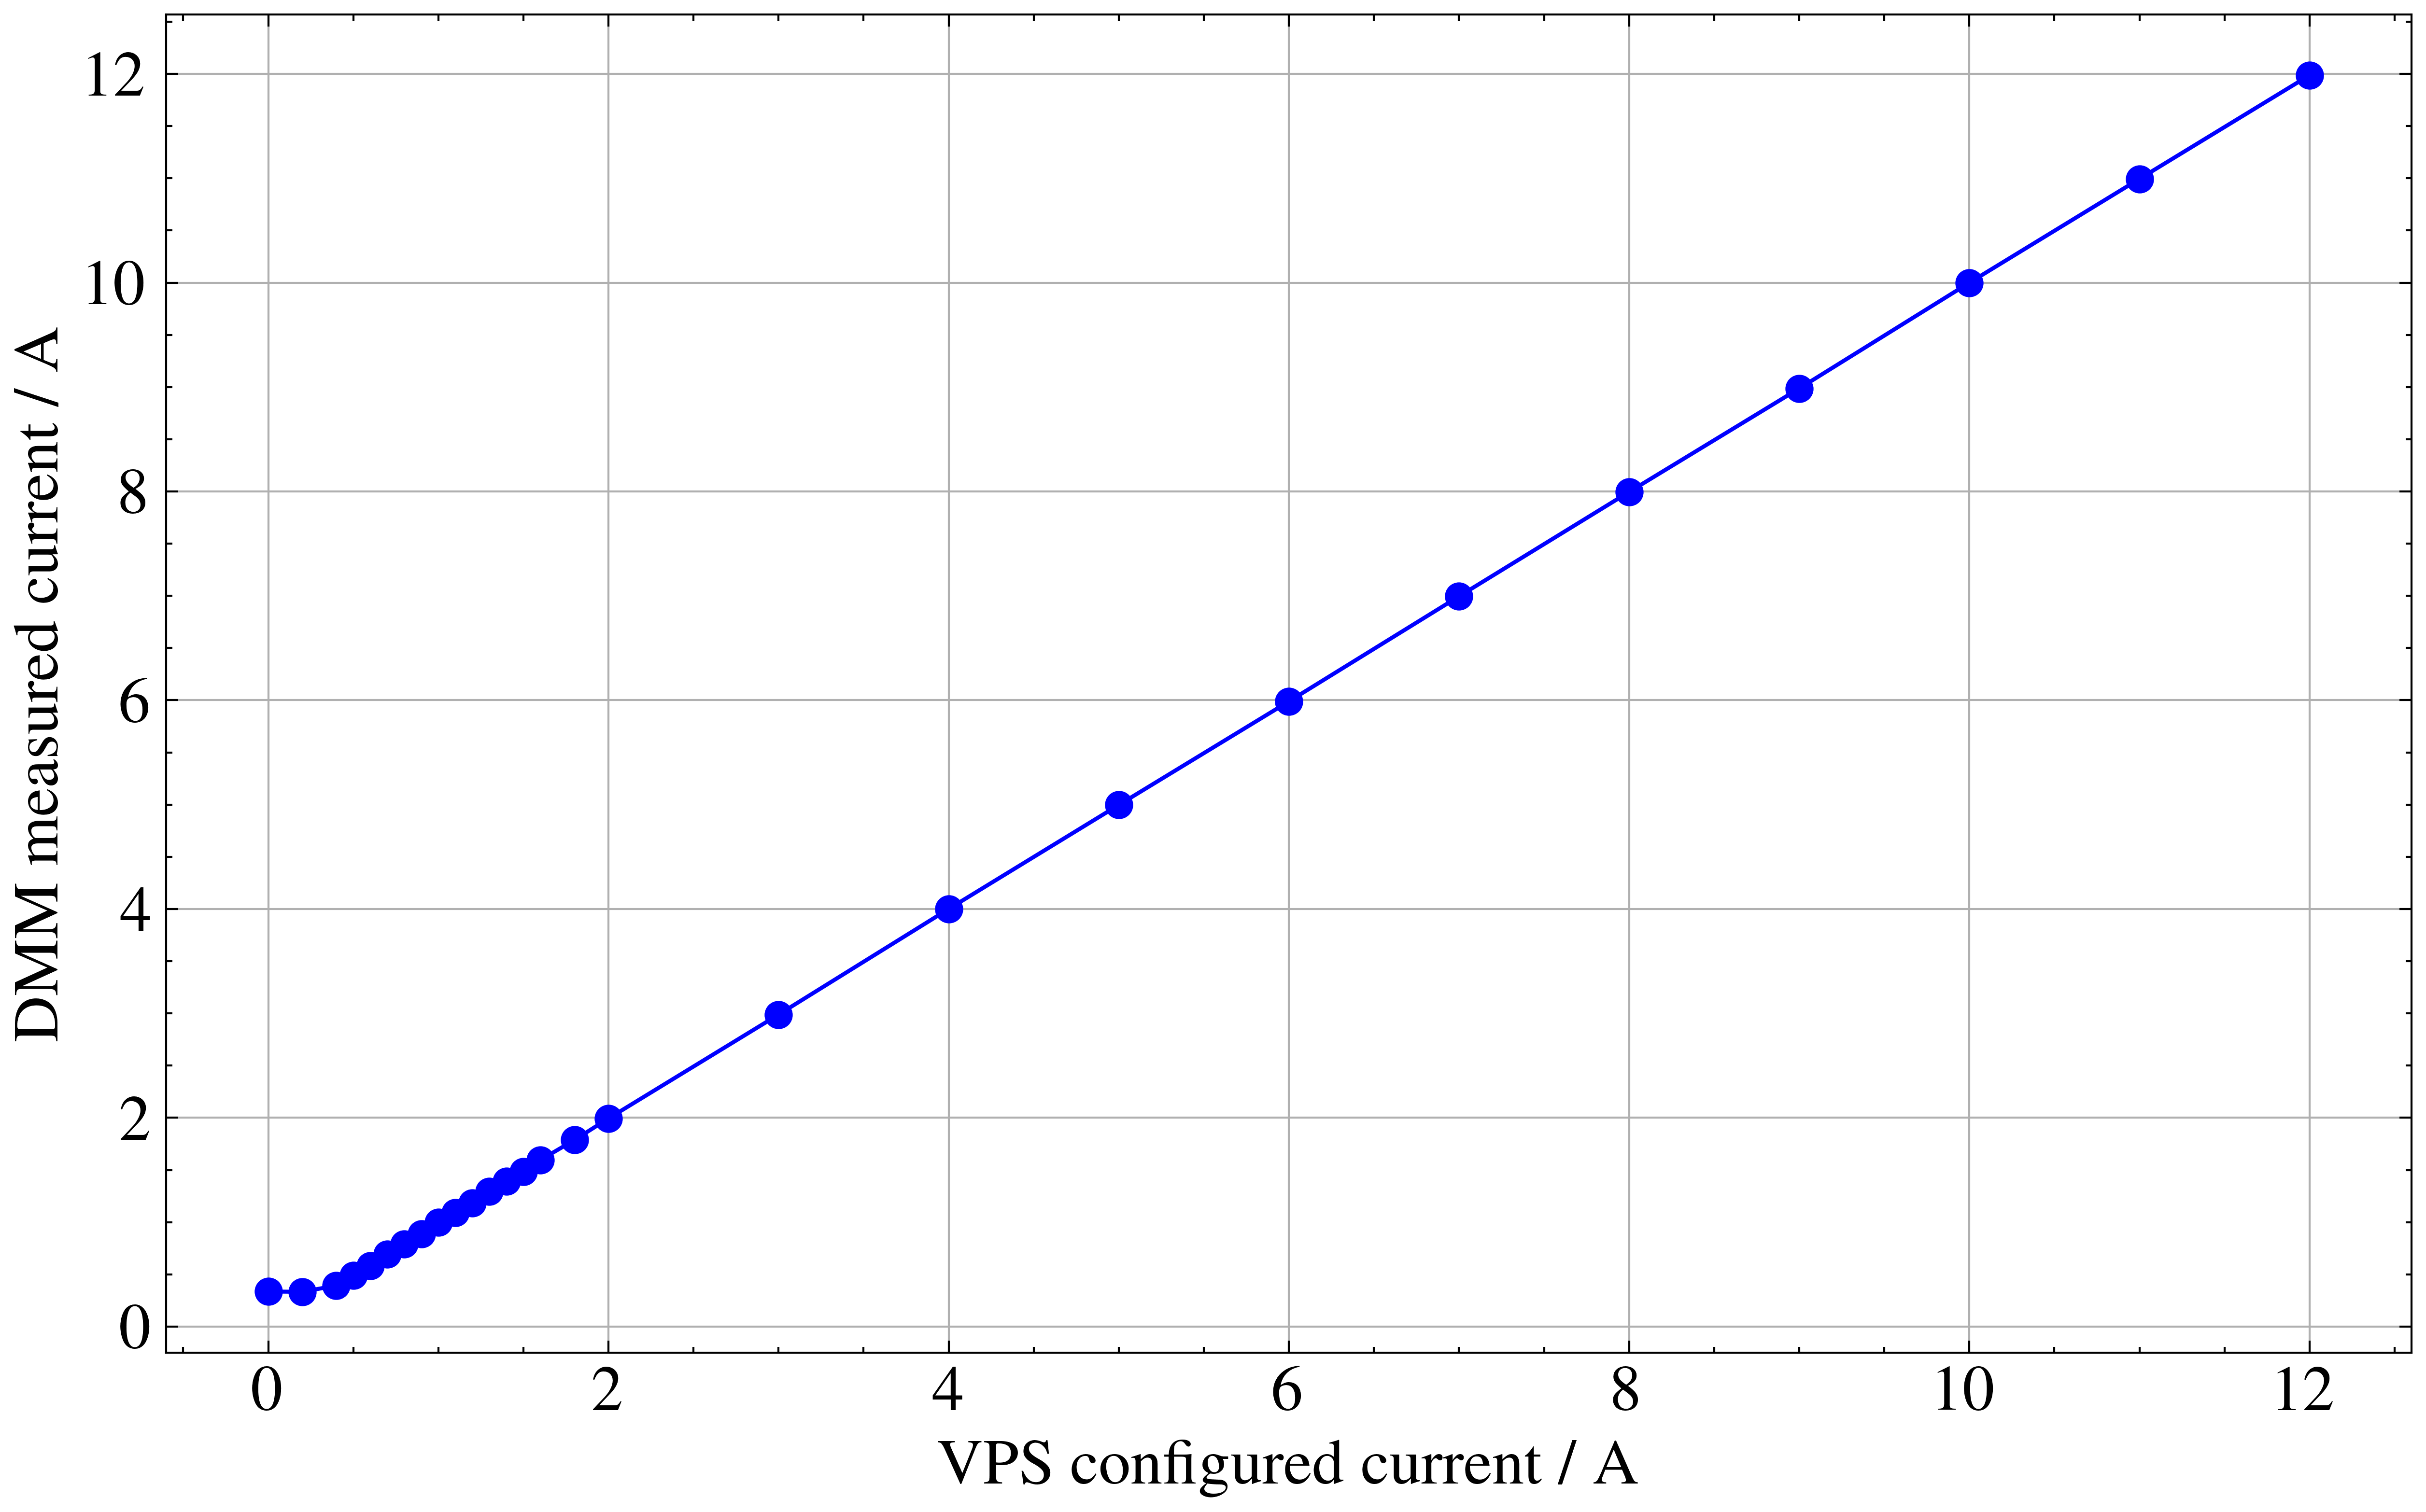
\includegraphics[width=0.6\textwidth]{src/figures/exp2/vps-dmm.png}
	\caption{VPSの設定電流とDMMによる測定値の関係}\label{fig:exp2}
\end{figure}


\subsection{実験3}
\ref{subsec:exp2}の状態から、VPSの出力を\SI{10}{k\ohm}の抵抗に接続しそれをオペアンプを負側の入力に接続した。
回路図を図\ref{fig:exp3-circuit}に示す。
\begin{figure}[!htb]
	\centering
	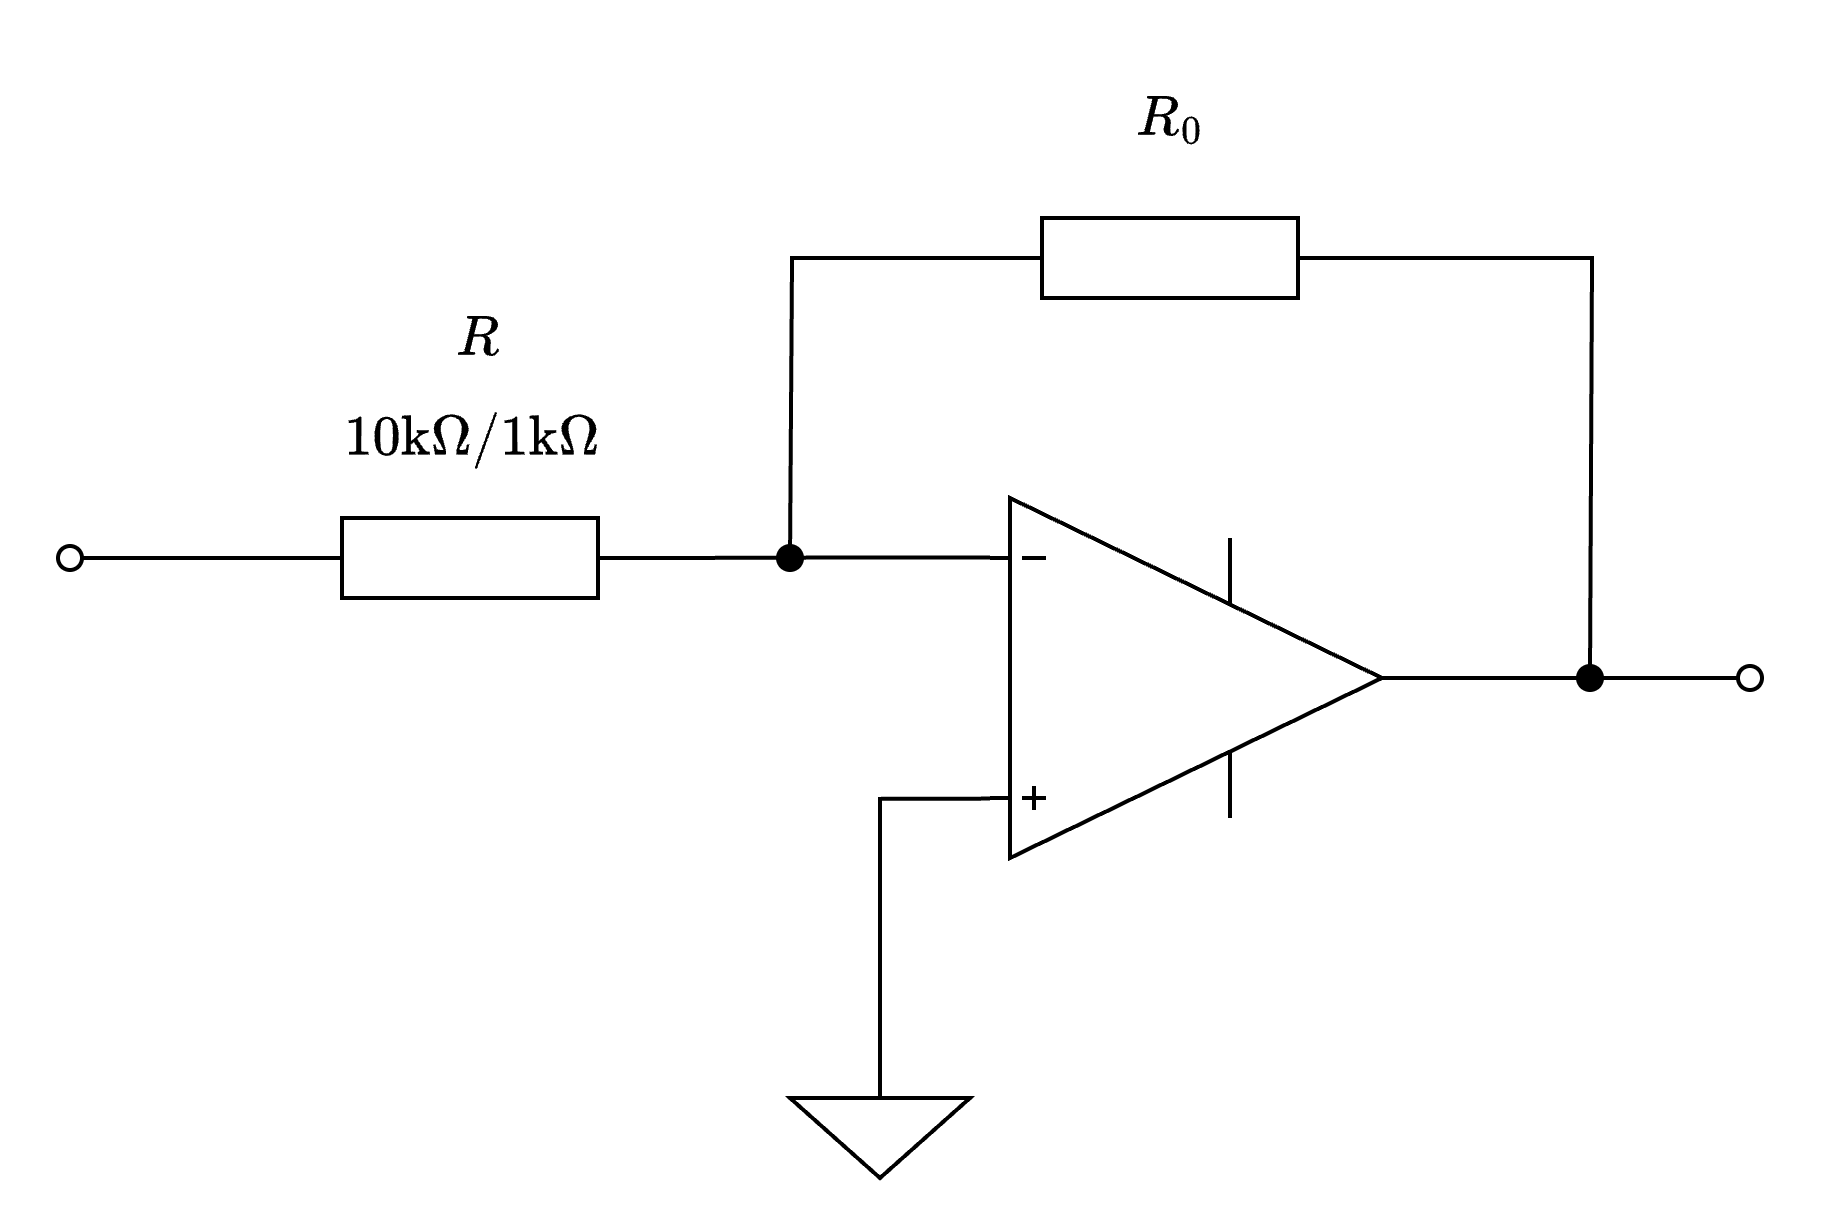
\includegraphics[width=0.6\linewidth]{src/figures/exp3/circuit.png}
	\caption{実験3 回路図}\label{fig:exp3-circuit}
\end{figure}

\ref{subsec:exp2}で測定したVPSの値を元に、\SI{0}{A}から\SI{12}{A}まで\SI{1}{A}刻みで変化させたときのオペアンプの出力を測定した。
また、VPSの出力を繋いだ抵抗の値を\SI{1}{k\ohm}に変更して、特に\SI{0}{A}から\SI{2}{A}までの間でオペアンプの出力を測定した。
この結果をそれぞれ表\ref{tab:exp3-10k}と表\ref{tab:exp3-1k}に示す。
これを元にグラフにしたものを図\ref{fig:exp3}に示す。
%Please add the following packages if necessary:
%\usepackage{booktabs, multirow} % for borders and merged ranges
%\usepackage{soul}% for underlines
%\usepackage[table]{xcolor} % for cell colors
%\usepackage{changepage,threeparttable} % for wide tables
%If the table is too wide, replace \begin{table}[!htp]...\end{table} with
%\begin{adjustwidth}{-2.5 cm}{-2.5 cm}\centering\begin{threeparttable}[!htb]...\end{threeparttable}\end{adjustwidth}
\begin{table}[!htp]\centering
	\caption{VPSの設定電流に対するオペアンプの出力電流 ($R=\SI{10}{k\ohm}$)}\label{tab:exp3-10k}
	\scriptsize
	\begin{tabular}{cc}\toprule
		VPSの設定電流 / \si{A} & オペアンプの出力電流 / \si{A} \\\midrule
		0                 & 0.31292             \\
		1                 & 0.9989              \\
		2                 & 2.0048              \\
		3                 & 3.0077              \\
		4                 & 4.0270              \\
		5                 & 5.0307              \\
		6                 & 6.0304              \\
		7                 & 7.0444              \\
		8                 & 8.0524              \\
		9                 & 9.0509              \\
		10                & 10.071              \\
		11                & 11.074              \\
		12                & 12.074              \\
		\bottomrule
	\end{tabular}
\end{table}

%Please add the following packages if necessary:
%\usepackage{booktabs, multirow} % for borders and merged ranges
%\usepackage{soul}% for underlines
%\usepackage[table]{xcolor} % for cell colors
%\usepackage{changepage,threeparttable} % for wide tables
%If the table is too wide, replace \begin{table}[!htp]...\end{table} with
%\begin{adjustwidth}{-2.5 cm}{-2.5 cm}\centering\begin{threeparttable}[!htb]...\end{threeparttable}\end{adjustwidth}
\begin{table}[!htp]\centering
	\caption{VPSの設定電流に対するオペアンプの出力電流 ($R=\SI{1}{k\ohm}$)}\label{tab:exp3-1k}
	\scriptsize
	\begin{tabular}{cc}\toprule
		VPSの設定電流 / A & オペアンプの出力電流 / A \\\midrule
		0            & -1.9330        \\
		0.2          & -1.9170        \\
		0.4          & -3.9645        \\
		0.6          & -5.9045        \\
		0.8          & -7.9931        \\
		1            & -10.065        \\
		1.2          & -11.988        \\
		1.4          & -13.170        \\
		1.6          & -13.182        \\
		1.8          & -13.181        \\
		2            & -13.180        \\
		\bottomrule
	\end{tabular}
\end{table}

\begin{figure}[!htp]
	\centering
	\begin{subfigure}{0.48\linewidth}
		\centering
		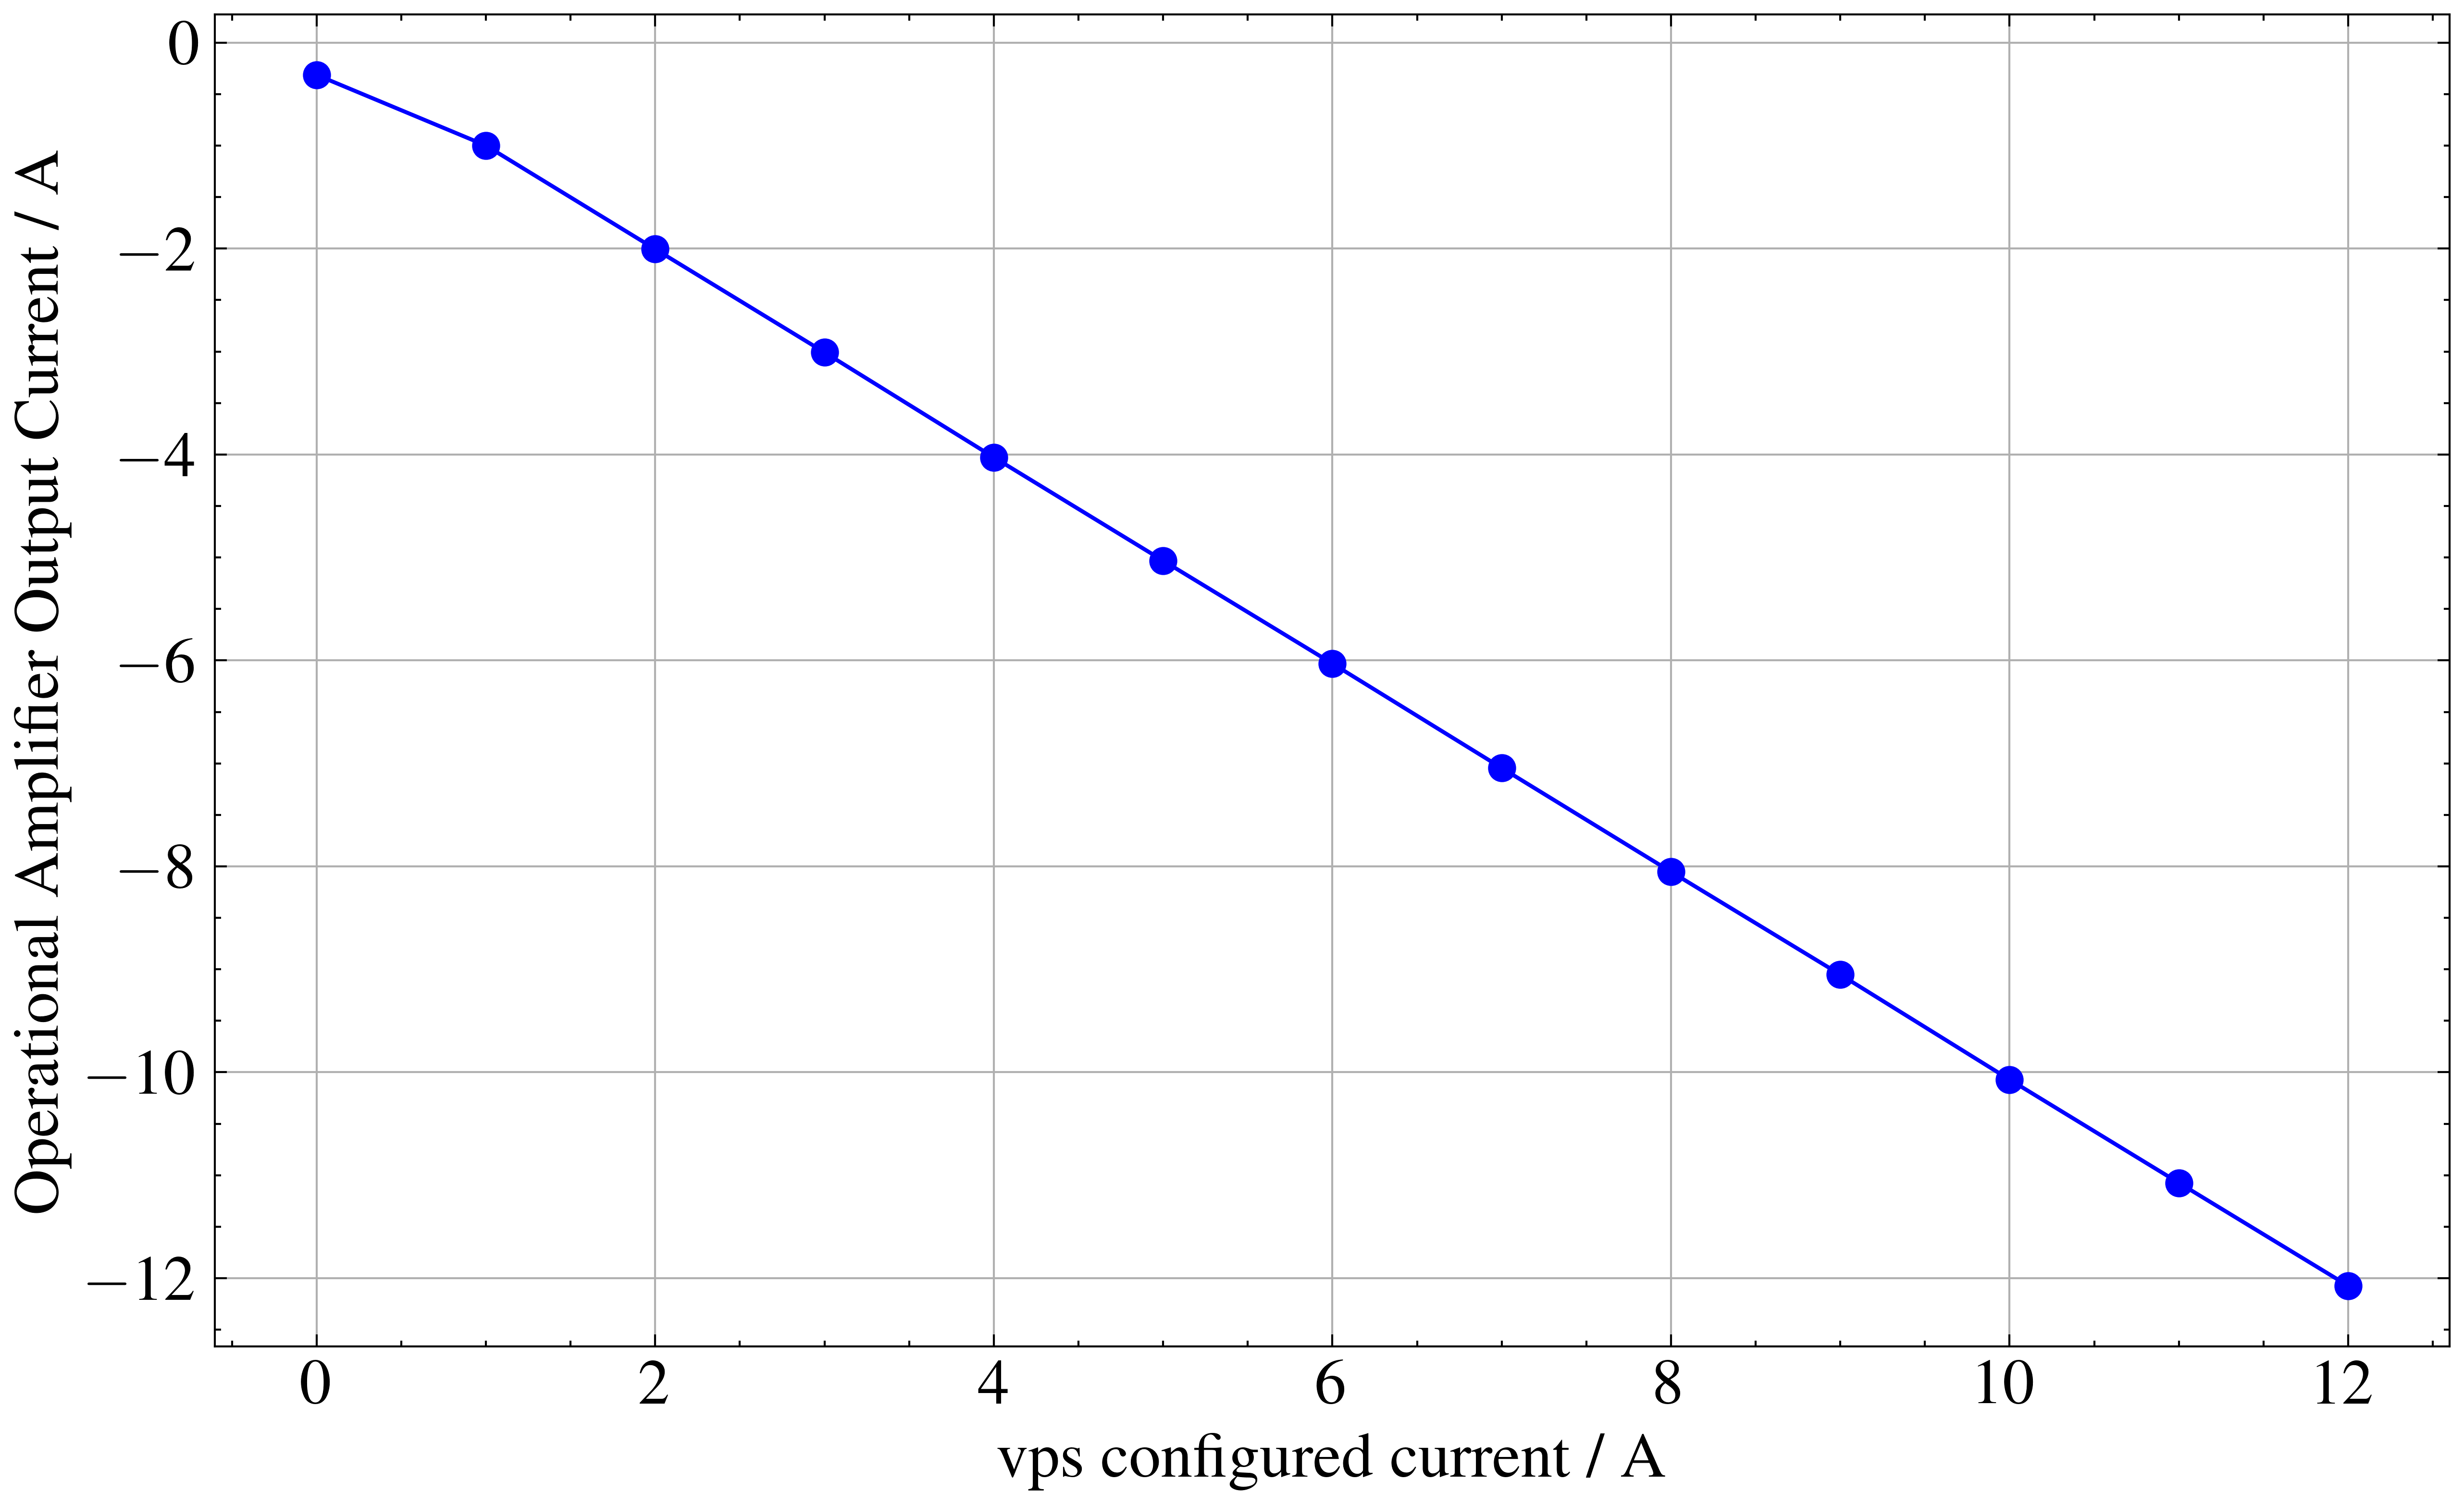
\includegraphics[width=0.8\linewidth]{src/figures/exp3/vps-op-amp-10k.png}
		\subcaption{$R=\SI{10}{k\ohm}$}\label{subfig:exp3-10k}
	\end{subfigure}
	\begin{subfigure}{0.48\linewidth}
		\centering
		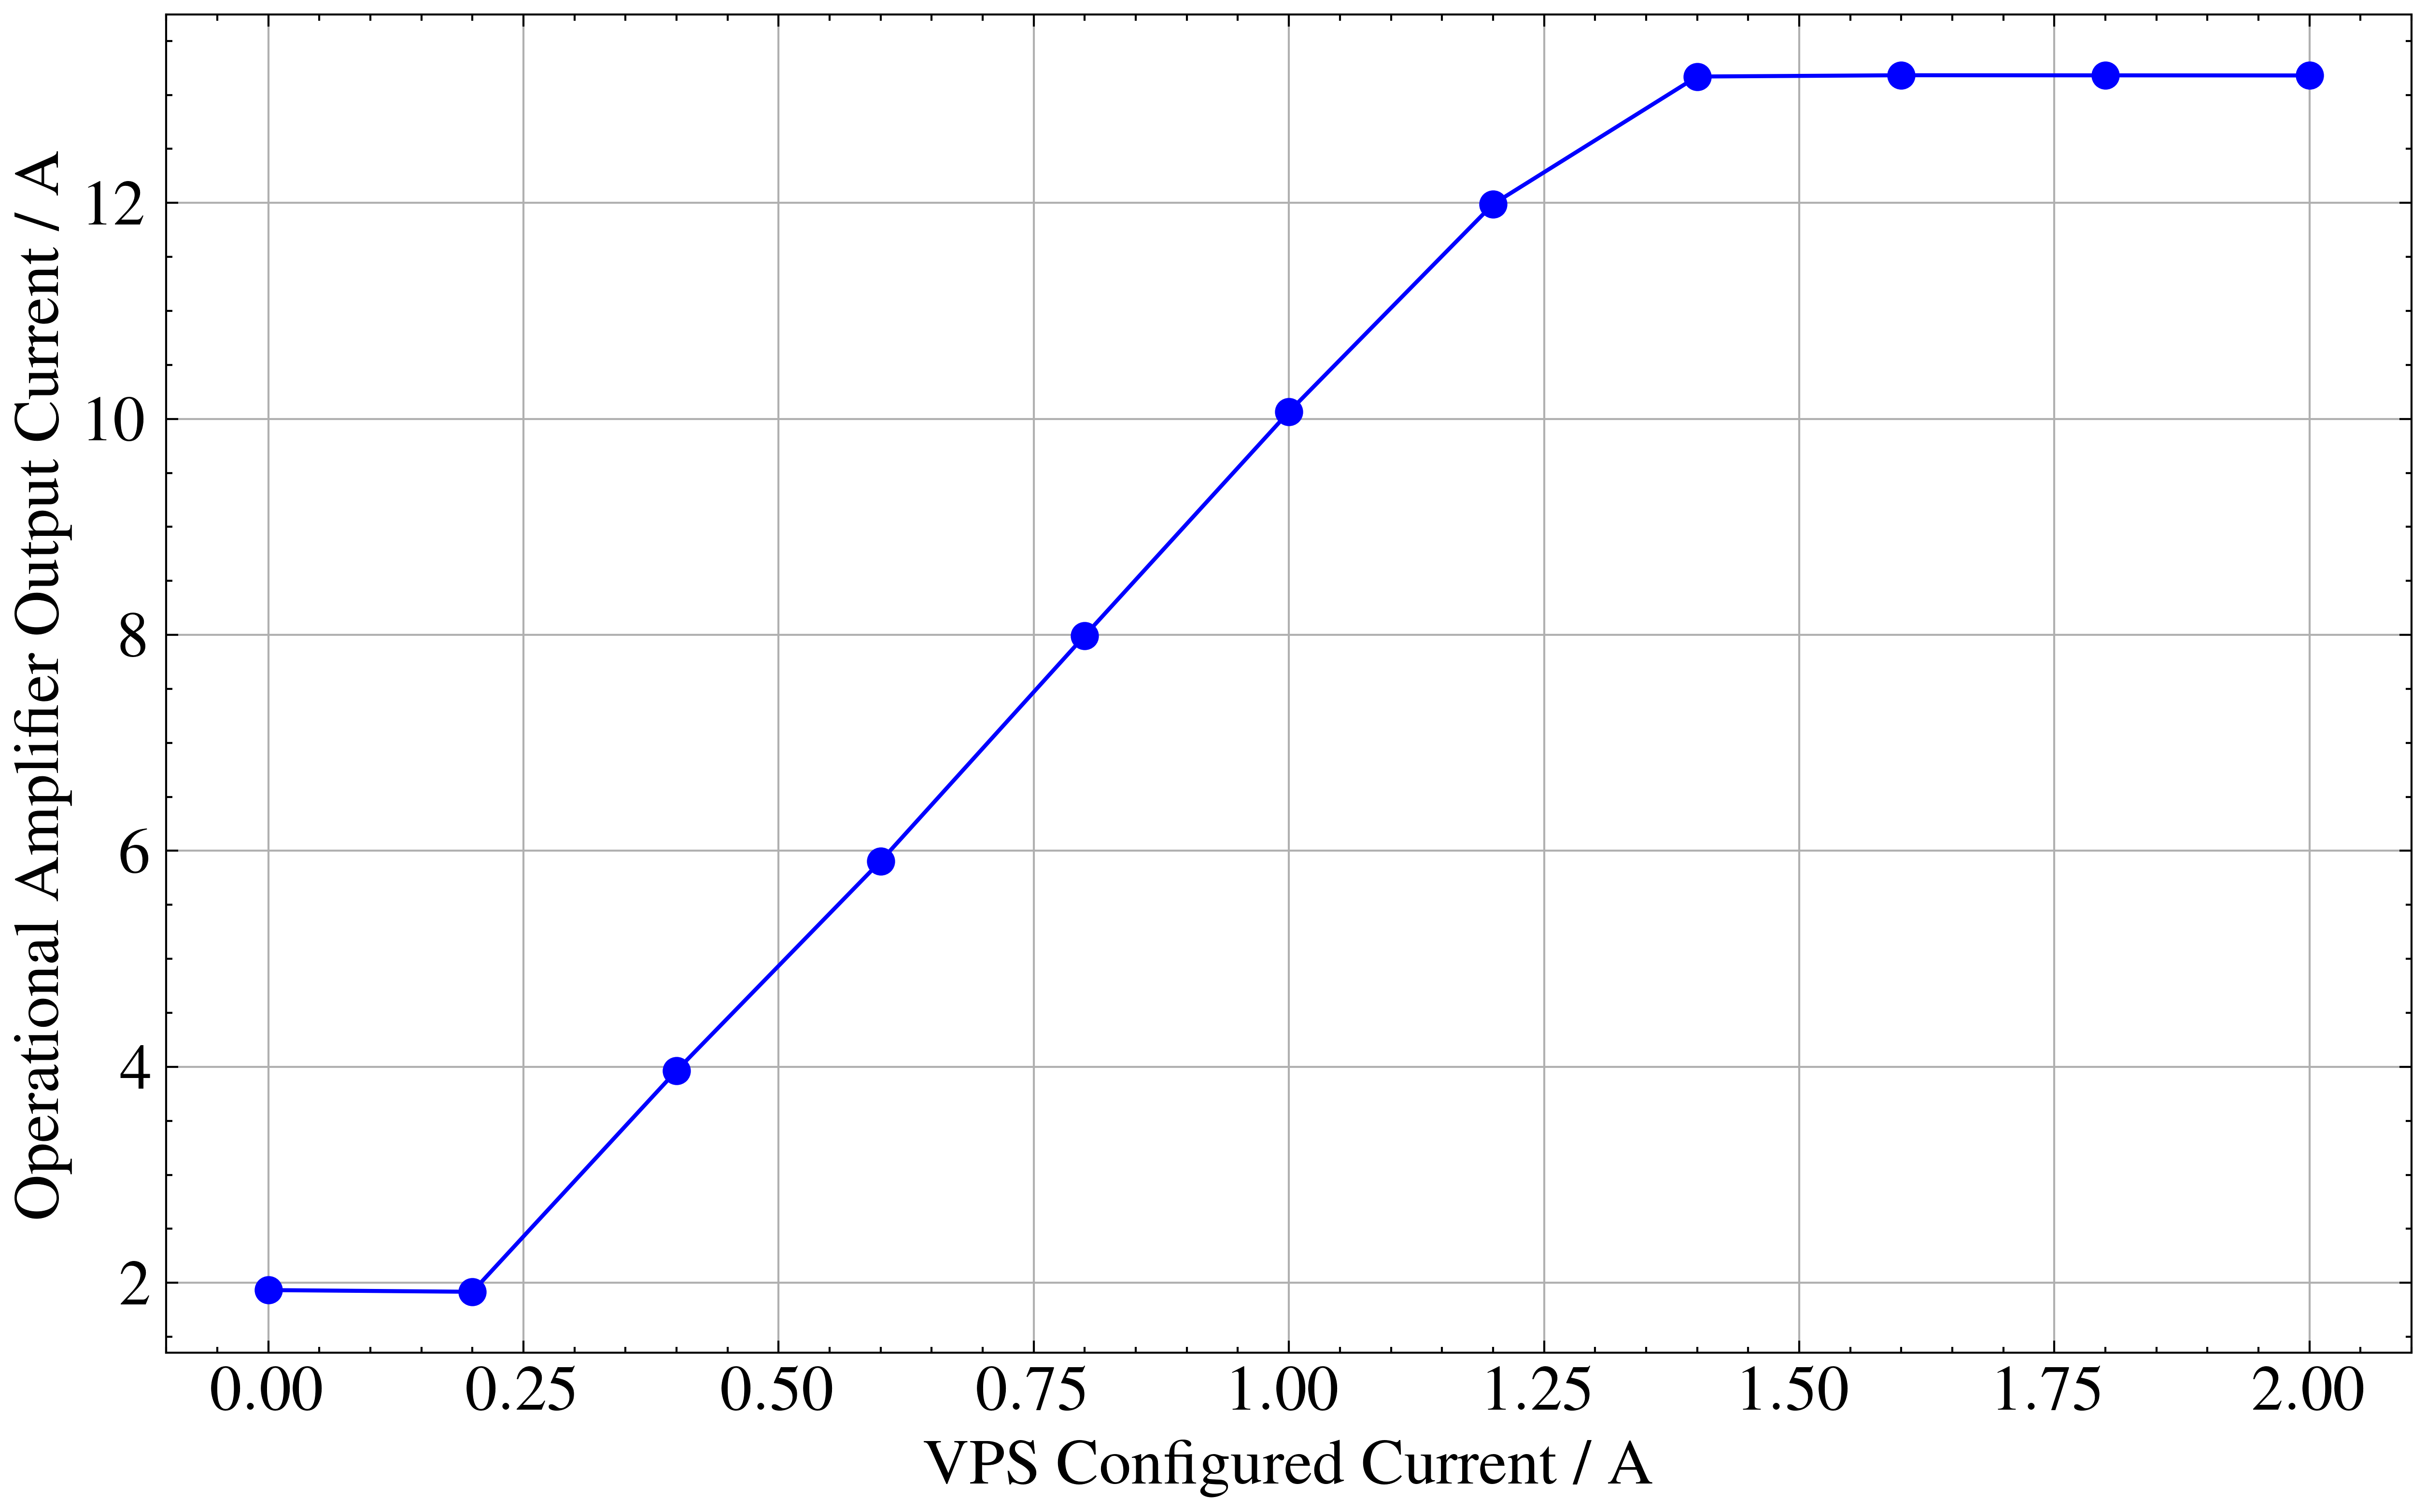
\includegraphics[width=0.8\linewidth]{src/figures/exp3/vps-op-amp-1k.png}
		\subcaption{$R=\SI{1}{k\ohm}$}\label{subfig:exp3-1k}
	\end{subfigure}
	\caption{VPSの設定電流に対するオペアンプの出力電流}\label{fig:exp3}
\end{figure}


\subsection{実験4}
太陽電池、フォトダイオードをオペアンプに入力しその出力にオシロスコープを接続し、LEDライトとMAGライトを点滅させたときの出力波形を撮影した。
また、太陽電池の実験室の照明(蛍光灯)下で出力波形を撮影した。
回路図の概略を図\ref{fig:exp4-circuit}に示す。
\begin{figure}[!htb]
	\centering
	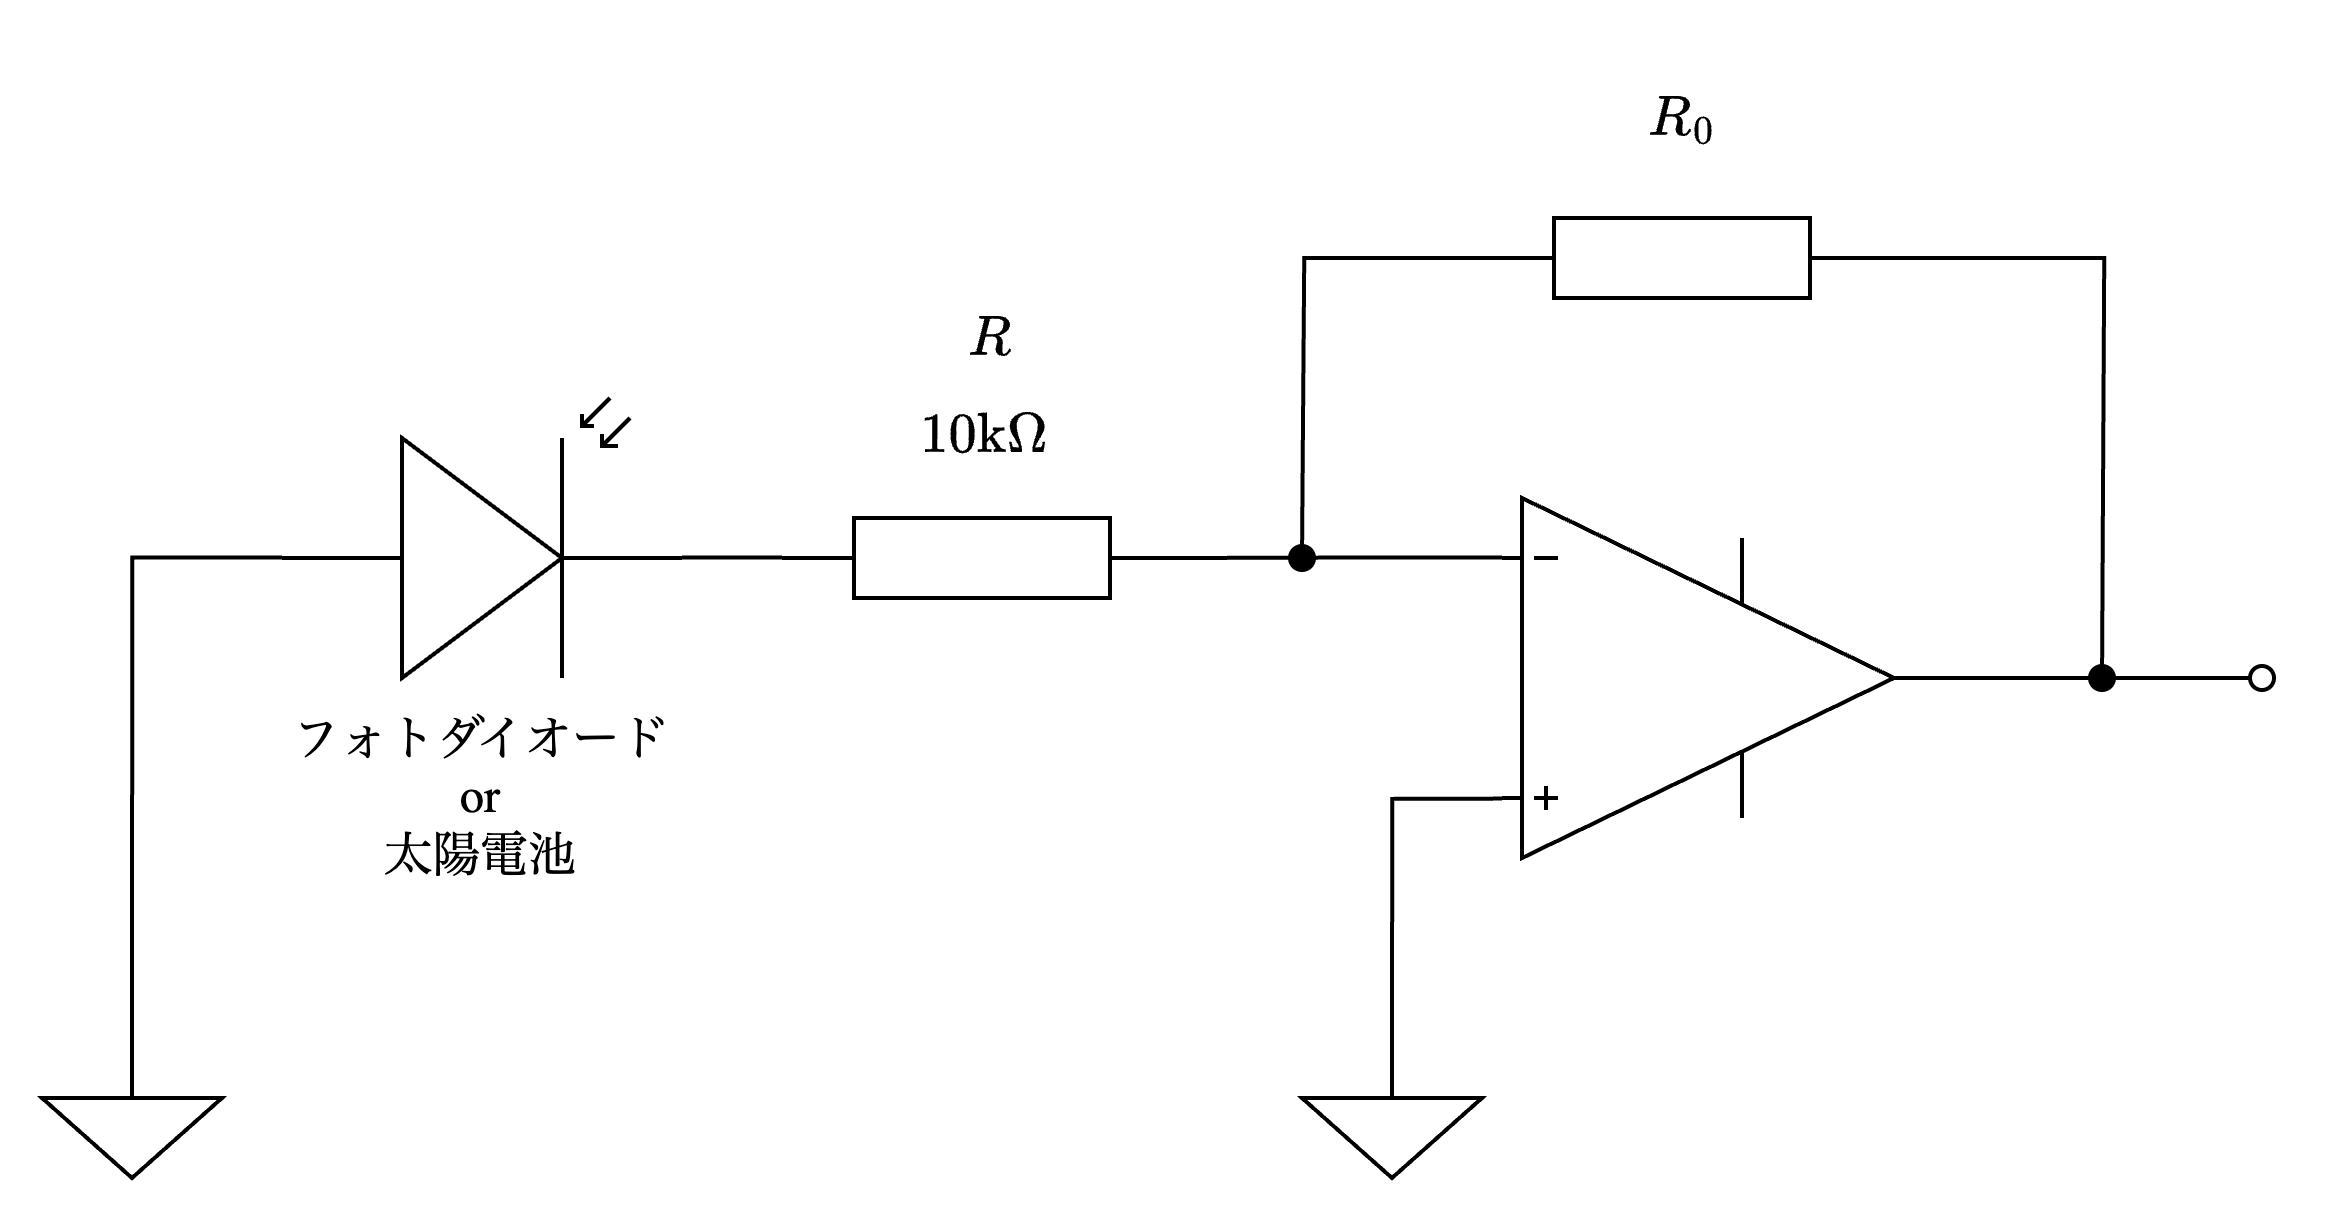
\includegraphics[width=0.6\linewidth]{src/figures/exp4/circuit.png}
	\caption{実験4 回路図}\label{fig:exp4-circuit}
\end{figure}

撮影した画像は\ref{fig:exp4-led}と\ref{fig:exp4-f-lamp}に示す。
LEDライトの点滅に対して太陽電池、フォトダイオードともにすぐに反応し矩形波状の波形が得られた。
図\ref{fig:exp4-led}から、LEDの波形の最大値は\SI{1.524}{V}、フォトダイオードは\SI{472.45}{mV}であった。
蛍光灯のもとでの太陽電池の出力波形は図\ref{fig:exp4-f-lamp}であり、周期的な波形が得られた。

\subsection{実験5}\label{subsec:exp5}
Function Generatorを用いて、オシロスコープのCH0に入力し正弦波・三角波・矩形波を表示させた。
正しく表示されたことを確認した。
次に、Function Generatorの出力を正弦波にして\SI{10}{k\ohm}または\SI{1}{k\ohm}の抵抗を介してオペアンプに接続しその出力をオシロスコープのCH1に入力した。
回路図を図\ref{fig:exp5-circuit}に示す。
撮影した波形は図\ref{fig:exp5-raw}に示す。
入力・出力の波形はどちらの場合でも正弦波状であった。
図\ref{fig:exp5-raw-10k}では、入力の振幅が\SI{1.027}{V}に対し出力の振幅は\SI{1.059}{V}であった。
図\ref{fig:exp5-raw-1k}では、入力の振幅が\SI{1.027}{V}に対し出力の振幅は\SI{9.876}{V}となった。
\begin{figure}
	\centering
	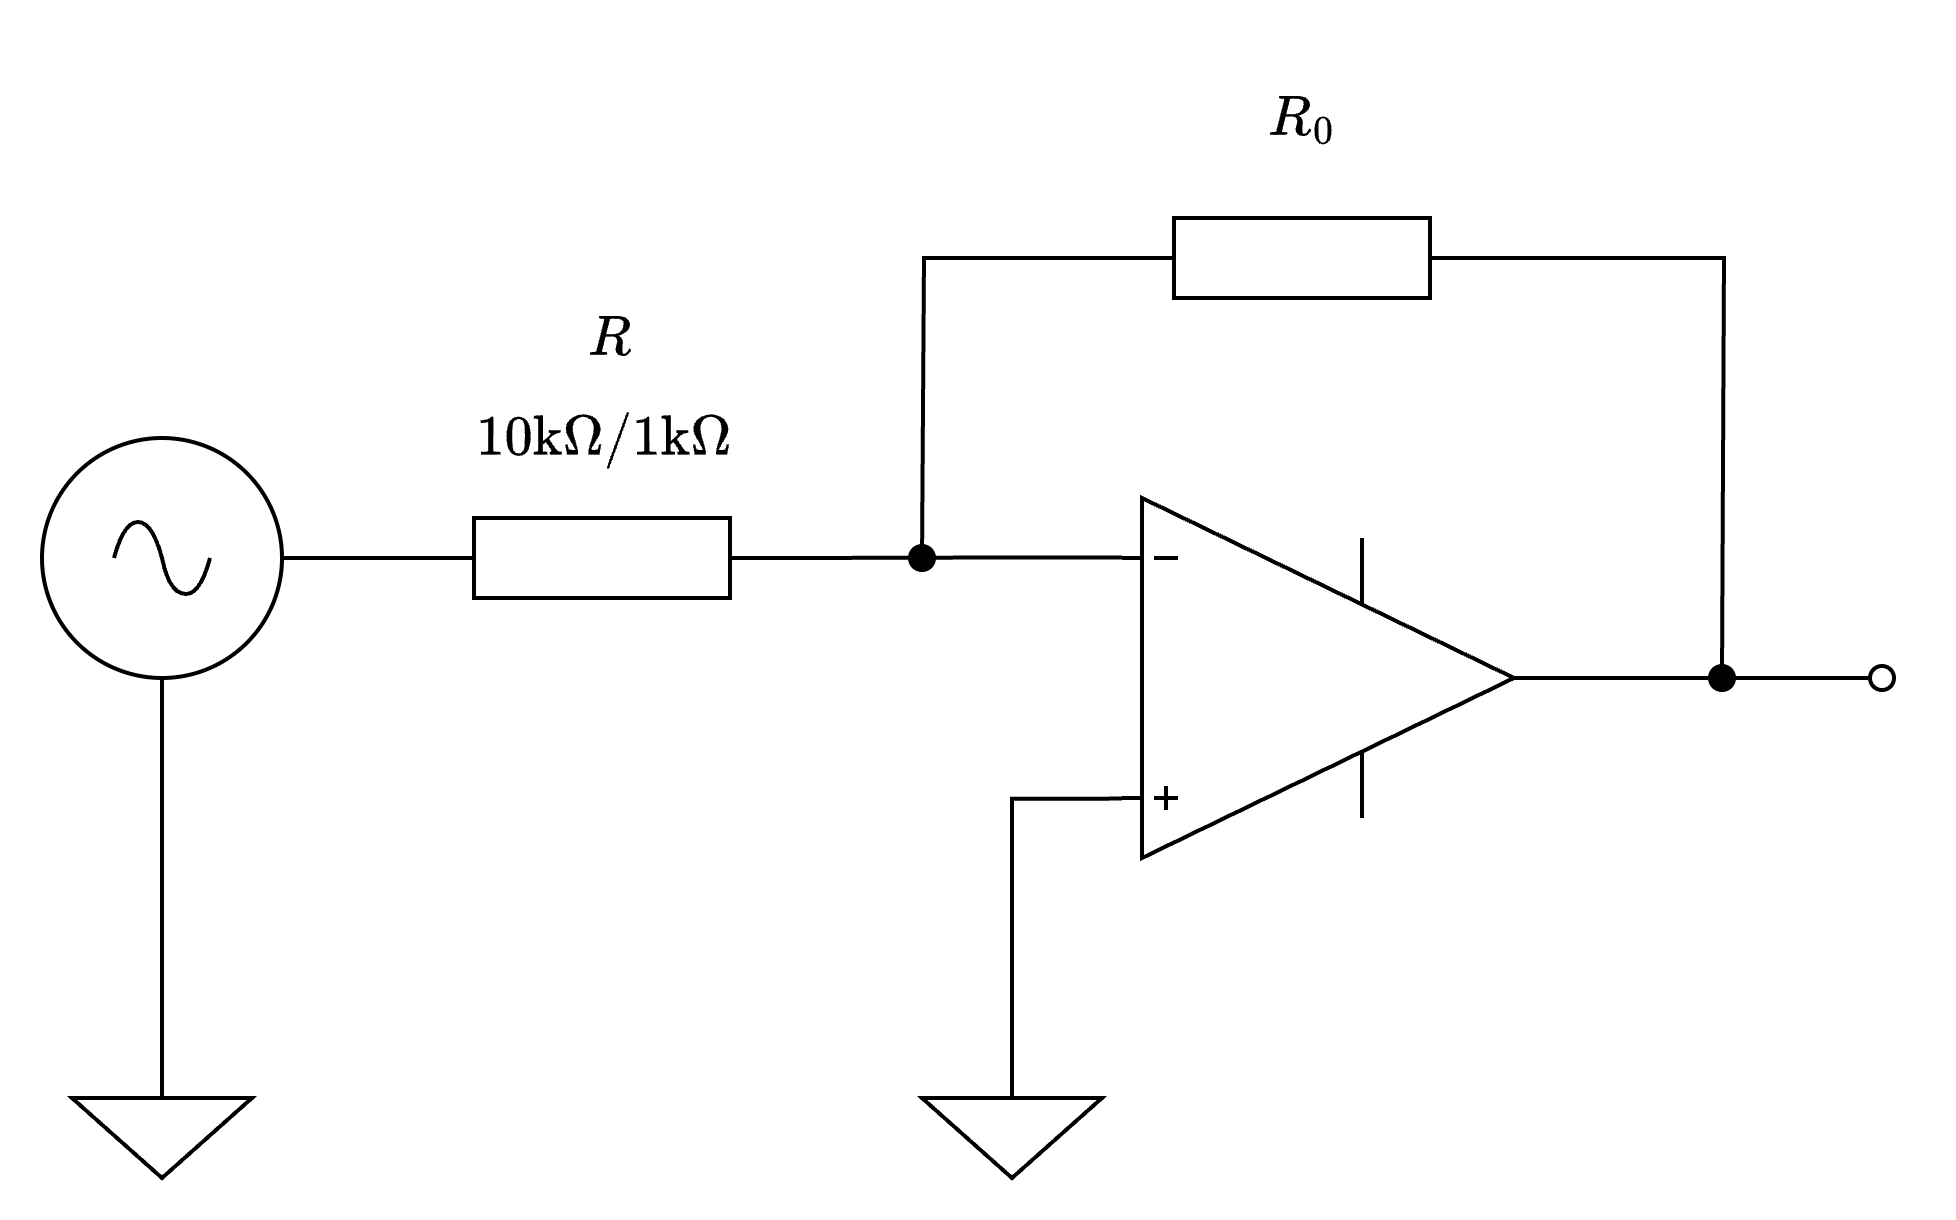
\includegraphics[width=0.6\linewidth]{src/figures/exp5/circuit.png}
	\caption{実験5 回路図}\label{fig:exp5-circuit}
\end{figure}


\subsection{実験6}
\ref{subsec:exp5}で接続していた抵抗$R$を\SI{0.1}{\micro\farad}のコンデンサに変更し、積分回路を作成した。
オペアンプの出力波形を測定した。
回路図の概略を図\ref{fig:exp6-circuit}に示す。
\begin{figure}[!htb]
    \centering
    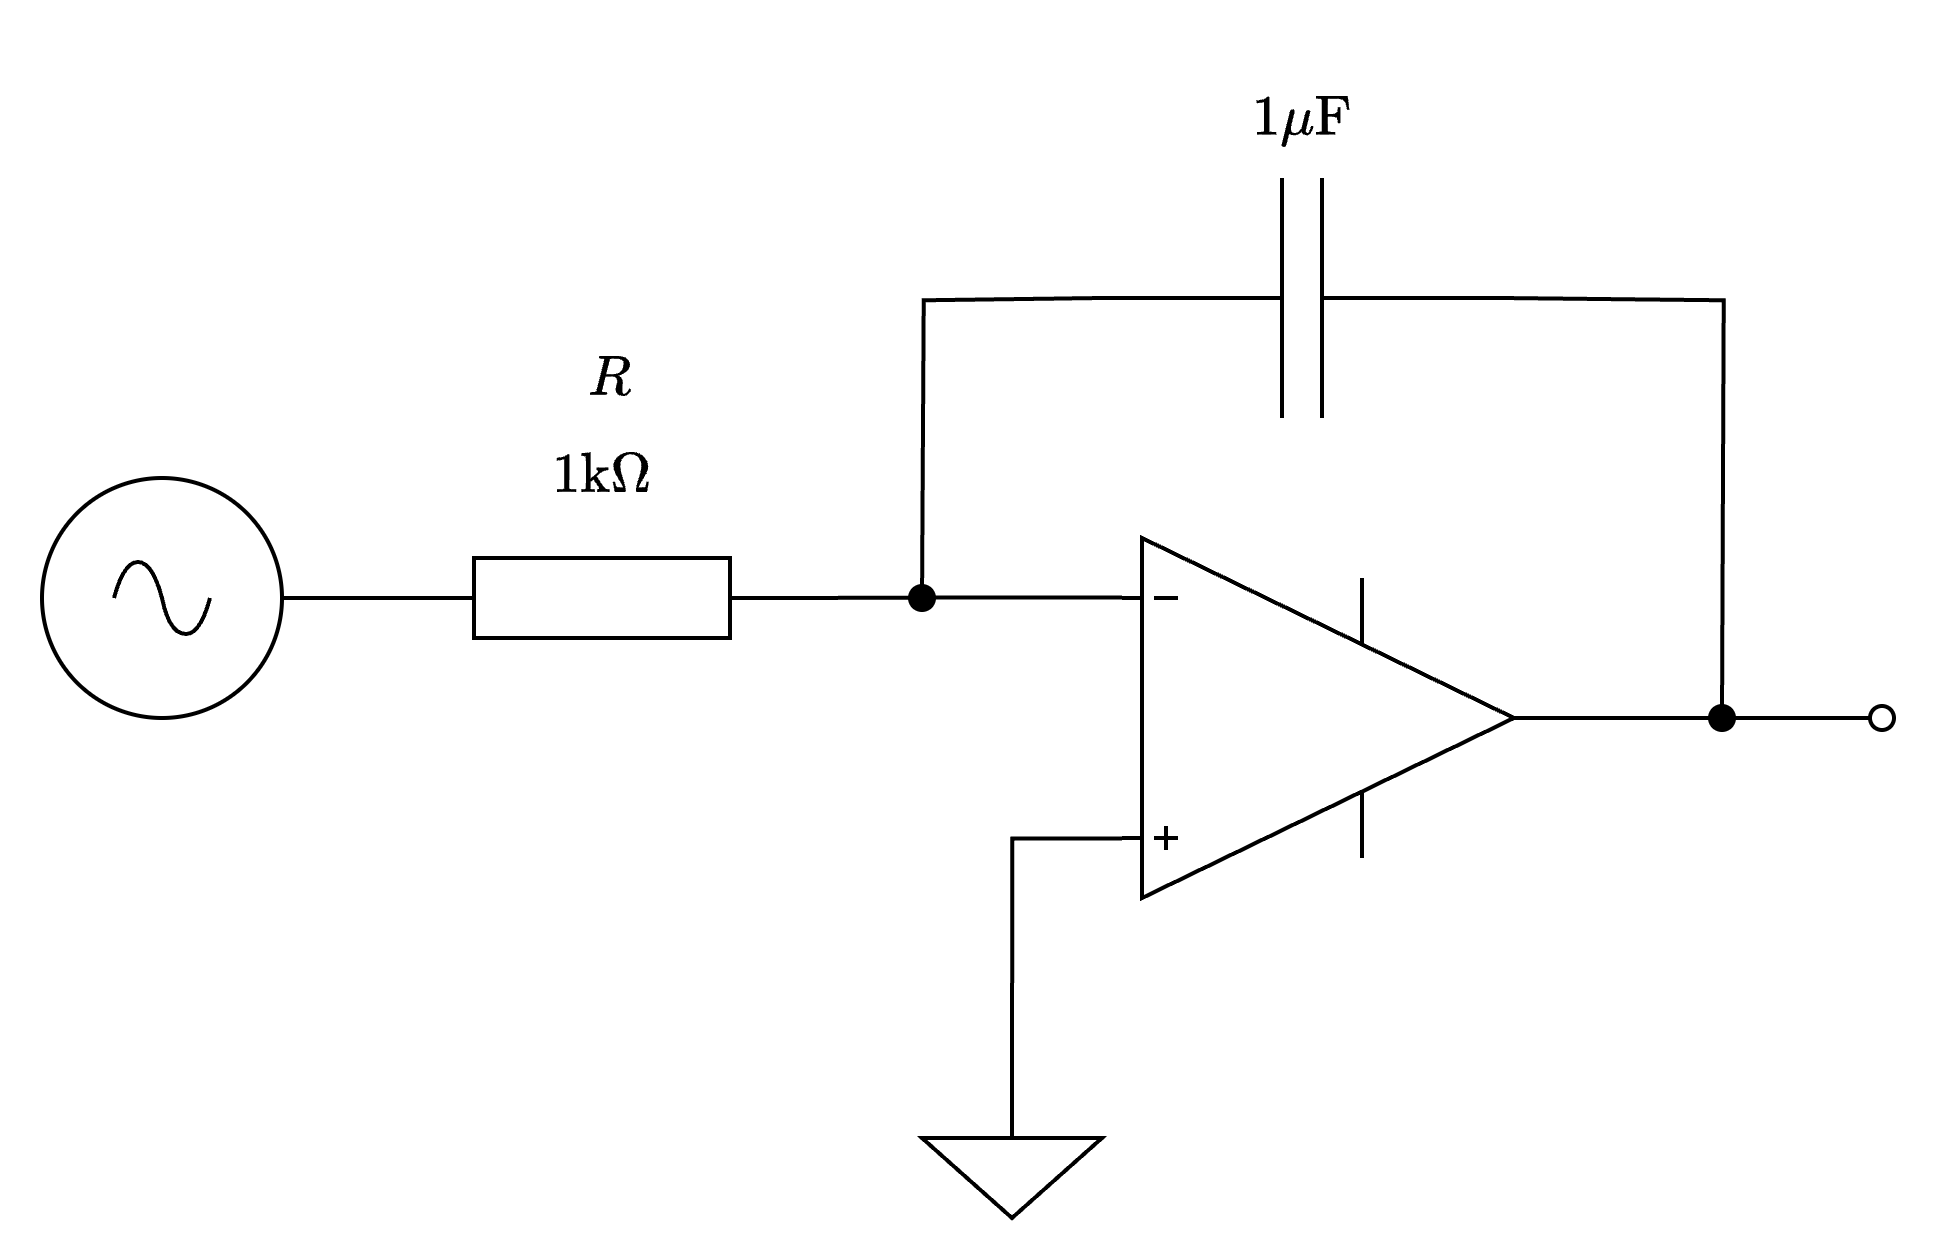
\includegraphics[width=0.6\linewidth]{src/figures/exp6/circuit.png}
    \caption{実験6 回路図}\label{fig:exp6-circuit}
\end{figure}

\begin{figure}[!htb]
    \centering
    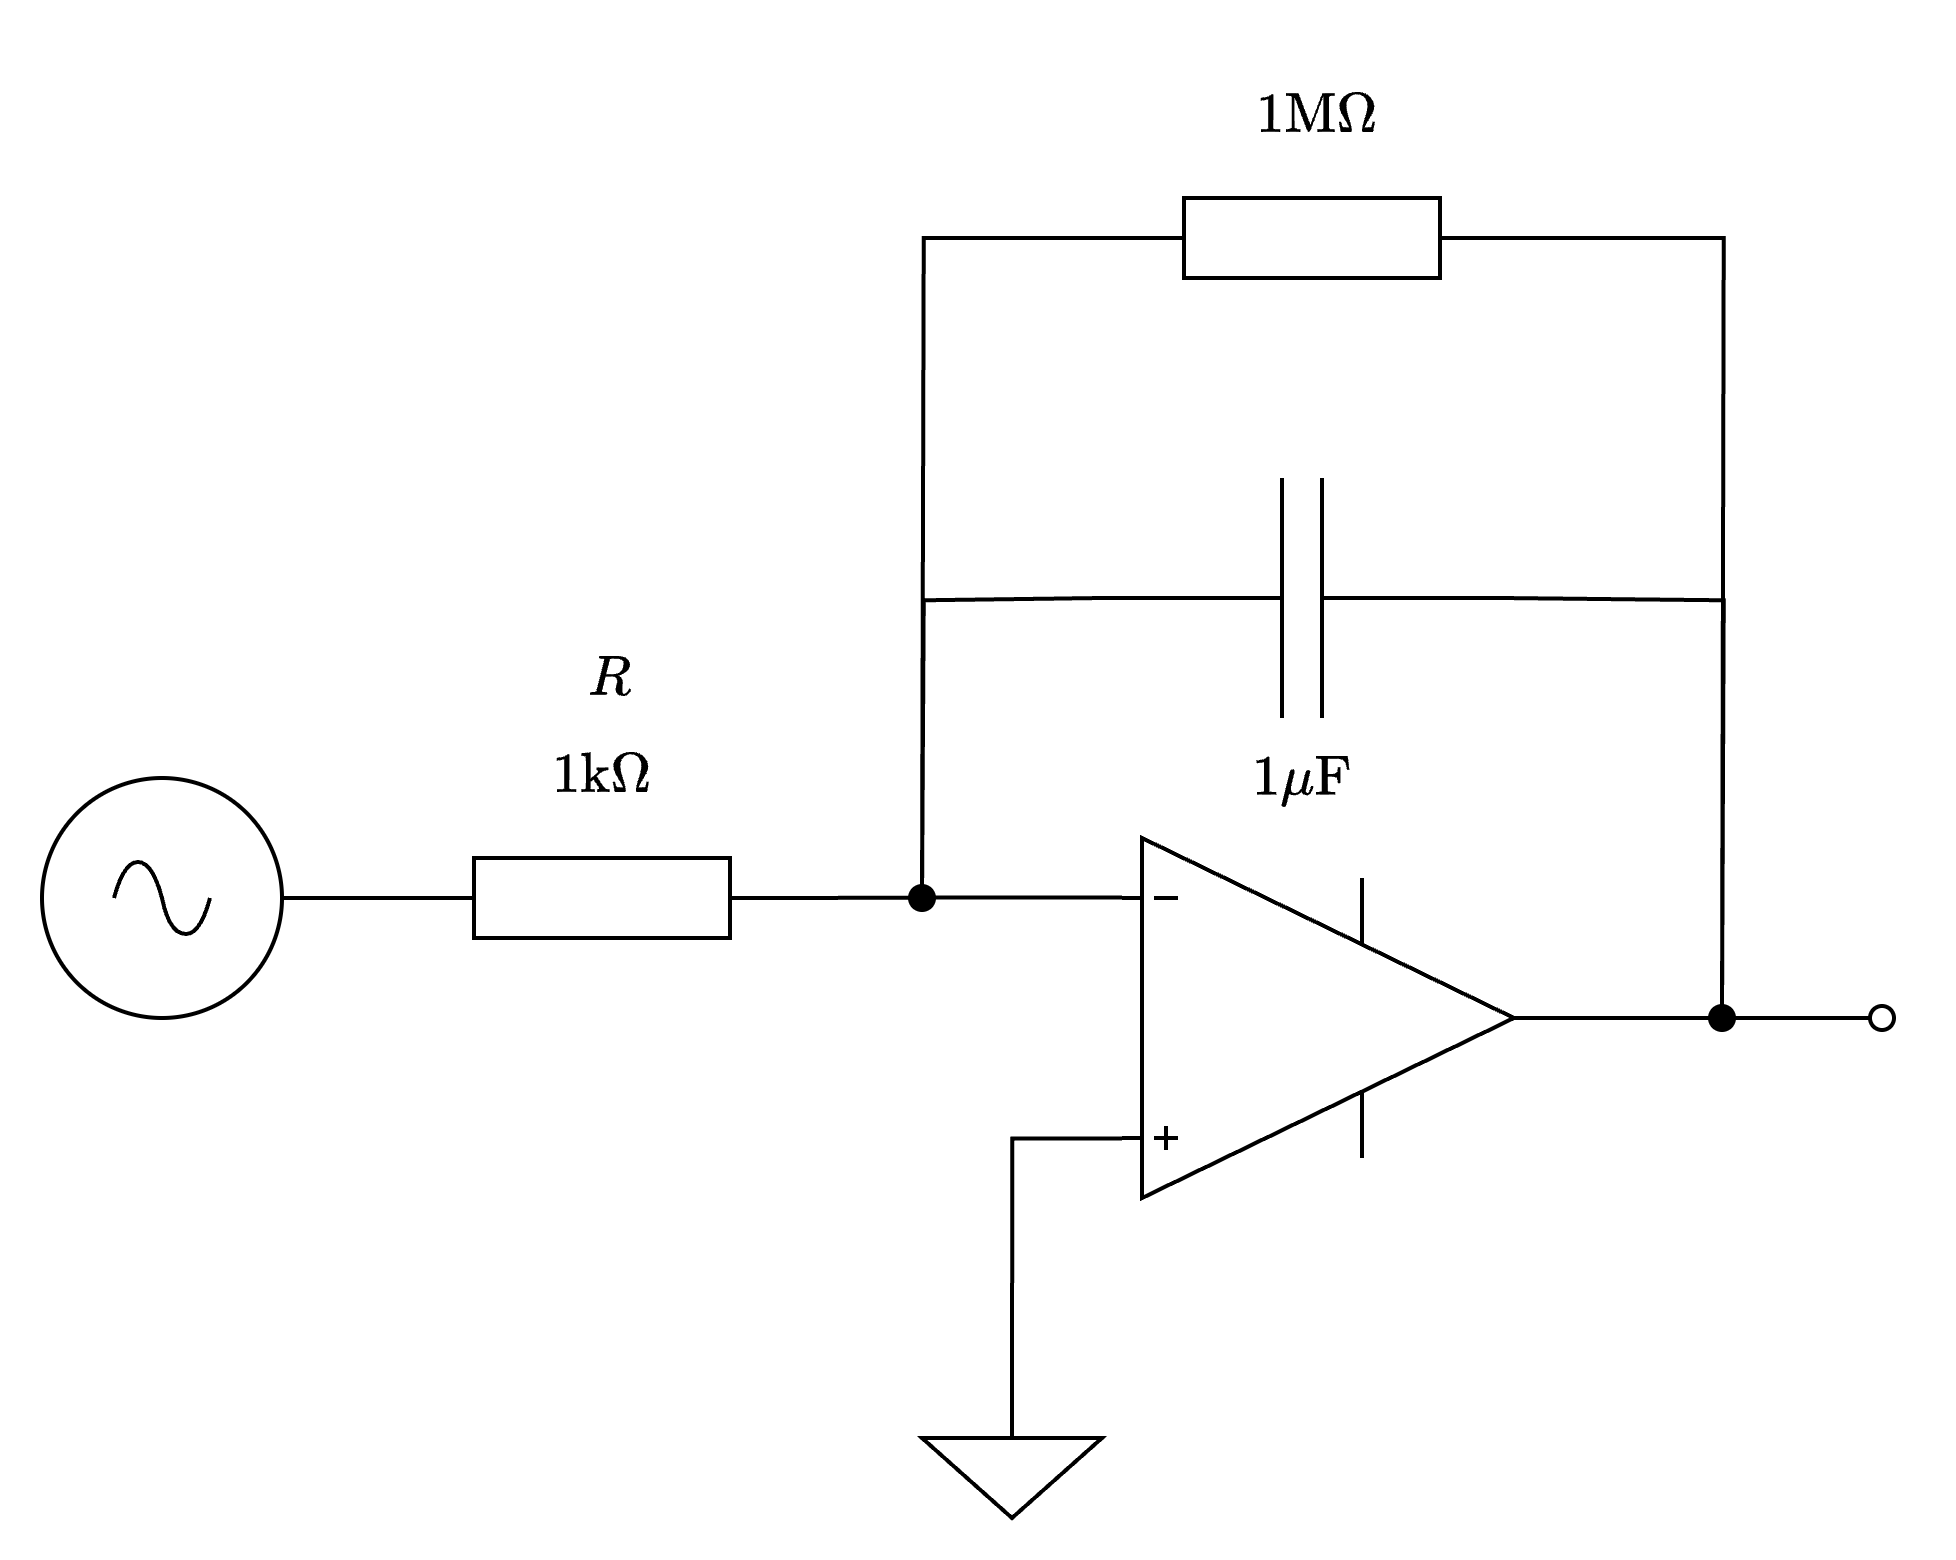
\includegraphics[width=0.6\linewidth]{src/figures/exp6/circuit2.png}
    \caption{実験6 回路図 2}\label{fig:exp6-circuit-2}
\end{figure}

この状態で\SI{20}{Hz}の矩形波を入力し、出力波形を観察した。
さらに、コンデンサに対して\SI{1}{M\ohm}の抵抗を接続し、\SI{20}{Hz}の矩形波・正弦波・三角波を入力し出力波形を観察した。
回路図は図\ref{fig:exp6-circuit-2}に示す。
撮影した画像は図\ref{fig:exp6-raw}に示す。
不完全積分回路に対して、矩形波を入力をした時は一定の部分で単調増加するような三角波の波形が得られた。
正弦波を入力したときは位相がずれた正弦波の出力が得られた。
三角波を入力したときは、正弦波のような波形が得られた。
積分回路と不完全積分回路に矩形波を入力した場合で比較すると、積分回路の方が出力された三角波状の波形が負側にずれている一方で、不完全積分回路ではほぼ振動中心は0に近い部分になっている。

\subsection{実験7}
図\ref{fig:exp7-circuit}に示すような加算回路を作成した。
\begin{figure}[!htb]
	\centering
	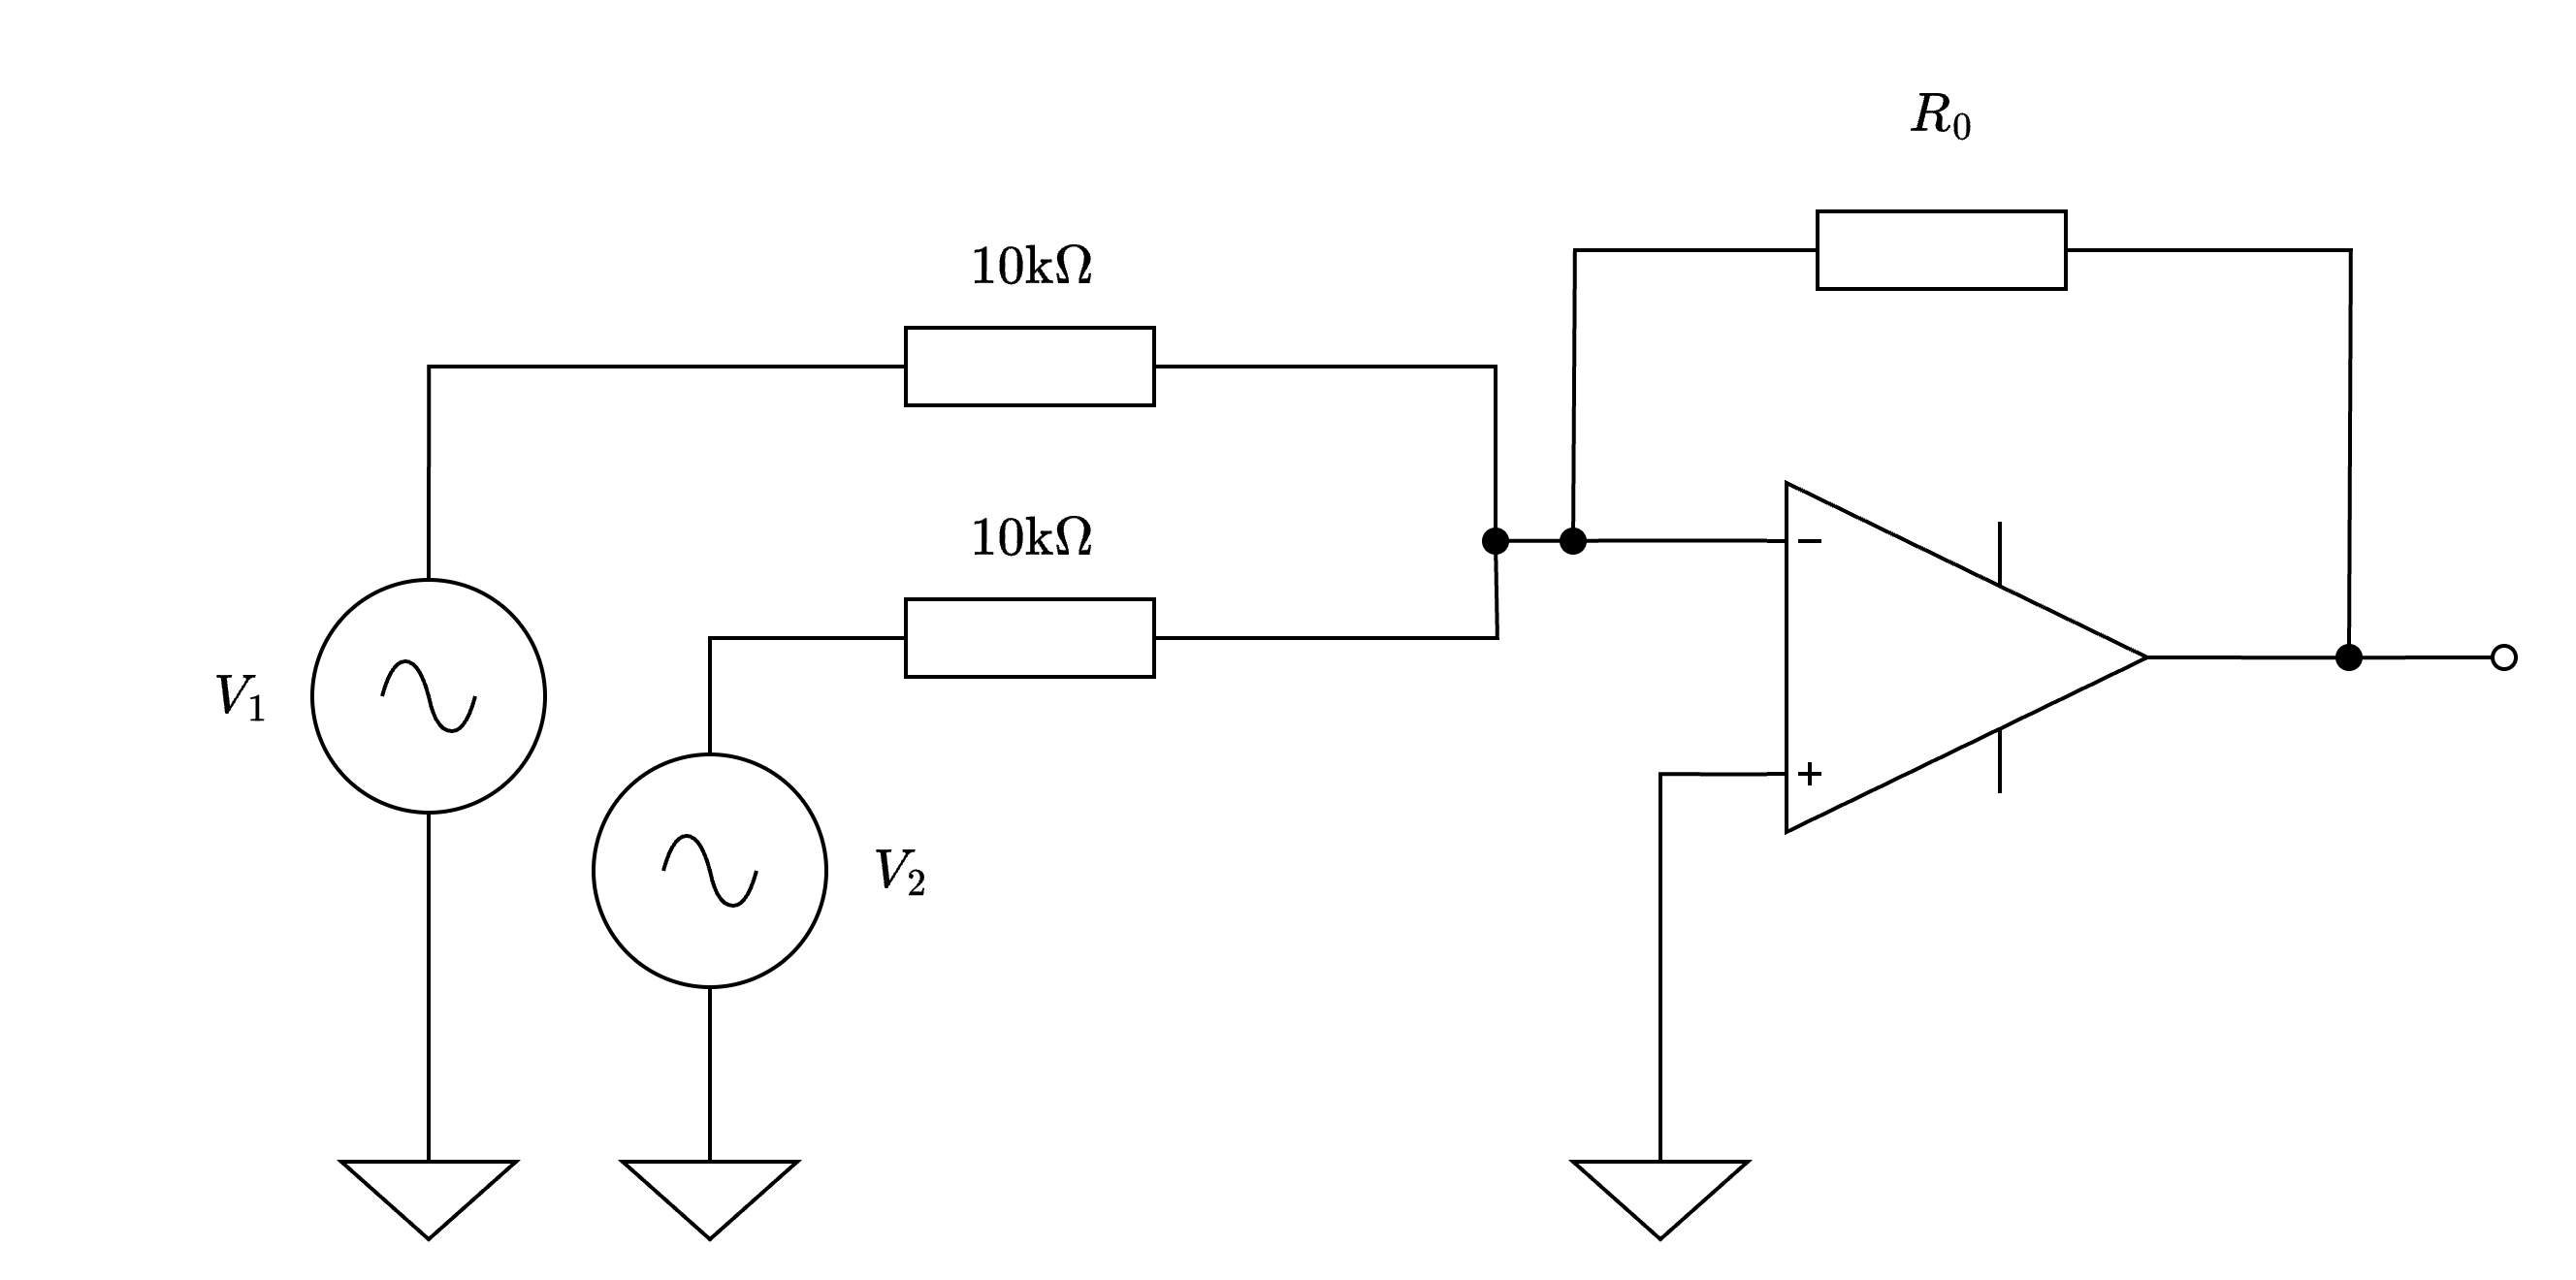
\includegraphics[width=0.7\linewidth]{src/figures/exp7/circuit.png}
	\caption{実験7 回路図}\label{fig:exp7-circuit}
\end{figure}

$V_1$、$V_2$として一方にはFunction Generatorから\SI{20}{Hz}の正弦波を入力し、もう一方にはVPSから\SI{0}{V}、\SI{1}{V}、\SI{2}{V}と変化させその波形を撮影した。
撮影した波形は図\ref{fig:exp7-raw}に示す。
VPSの電流を大きくするにつれて、出力波形は負側にシフトしていっていることがわかる。
VPSが\SI{0}{V}のとき、図\ref{fig:exp7-raw-0}より入力波形と出力波形は反転しているが、振幅は\SI{1.070}{V}と{1.059}{V}、振動数は\SI{19.898}{Hz}と\SI{19.867}{Hz}でほぼ一致している。
\SI{1}{V}のとき、図\ref{fig:exp7-raw-1}より出力波形の最大値が入力波形の最小値でありおおよそ\SI{1}{V}負側にシフトしているとわかる。


\subsection{実験8}\label{subsec:exp8}
図\ref{fig:exp8-circuit}に示すローパスフィルターを作成した。
\begin{figure}[!htb]
	\centering
	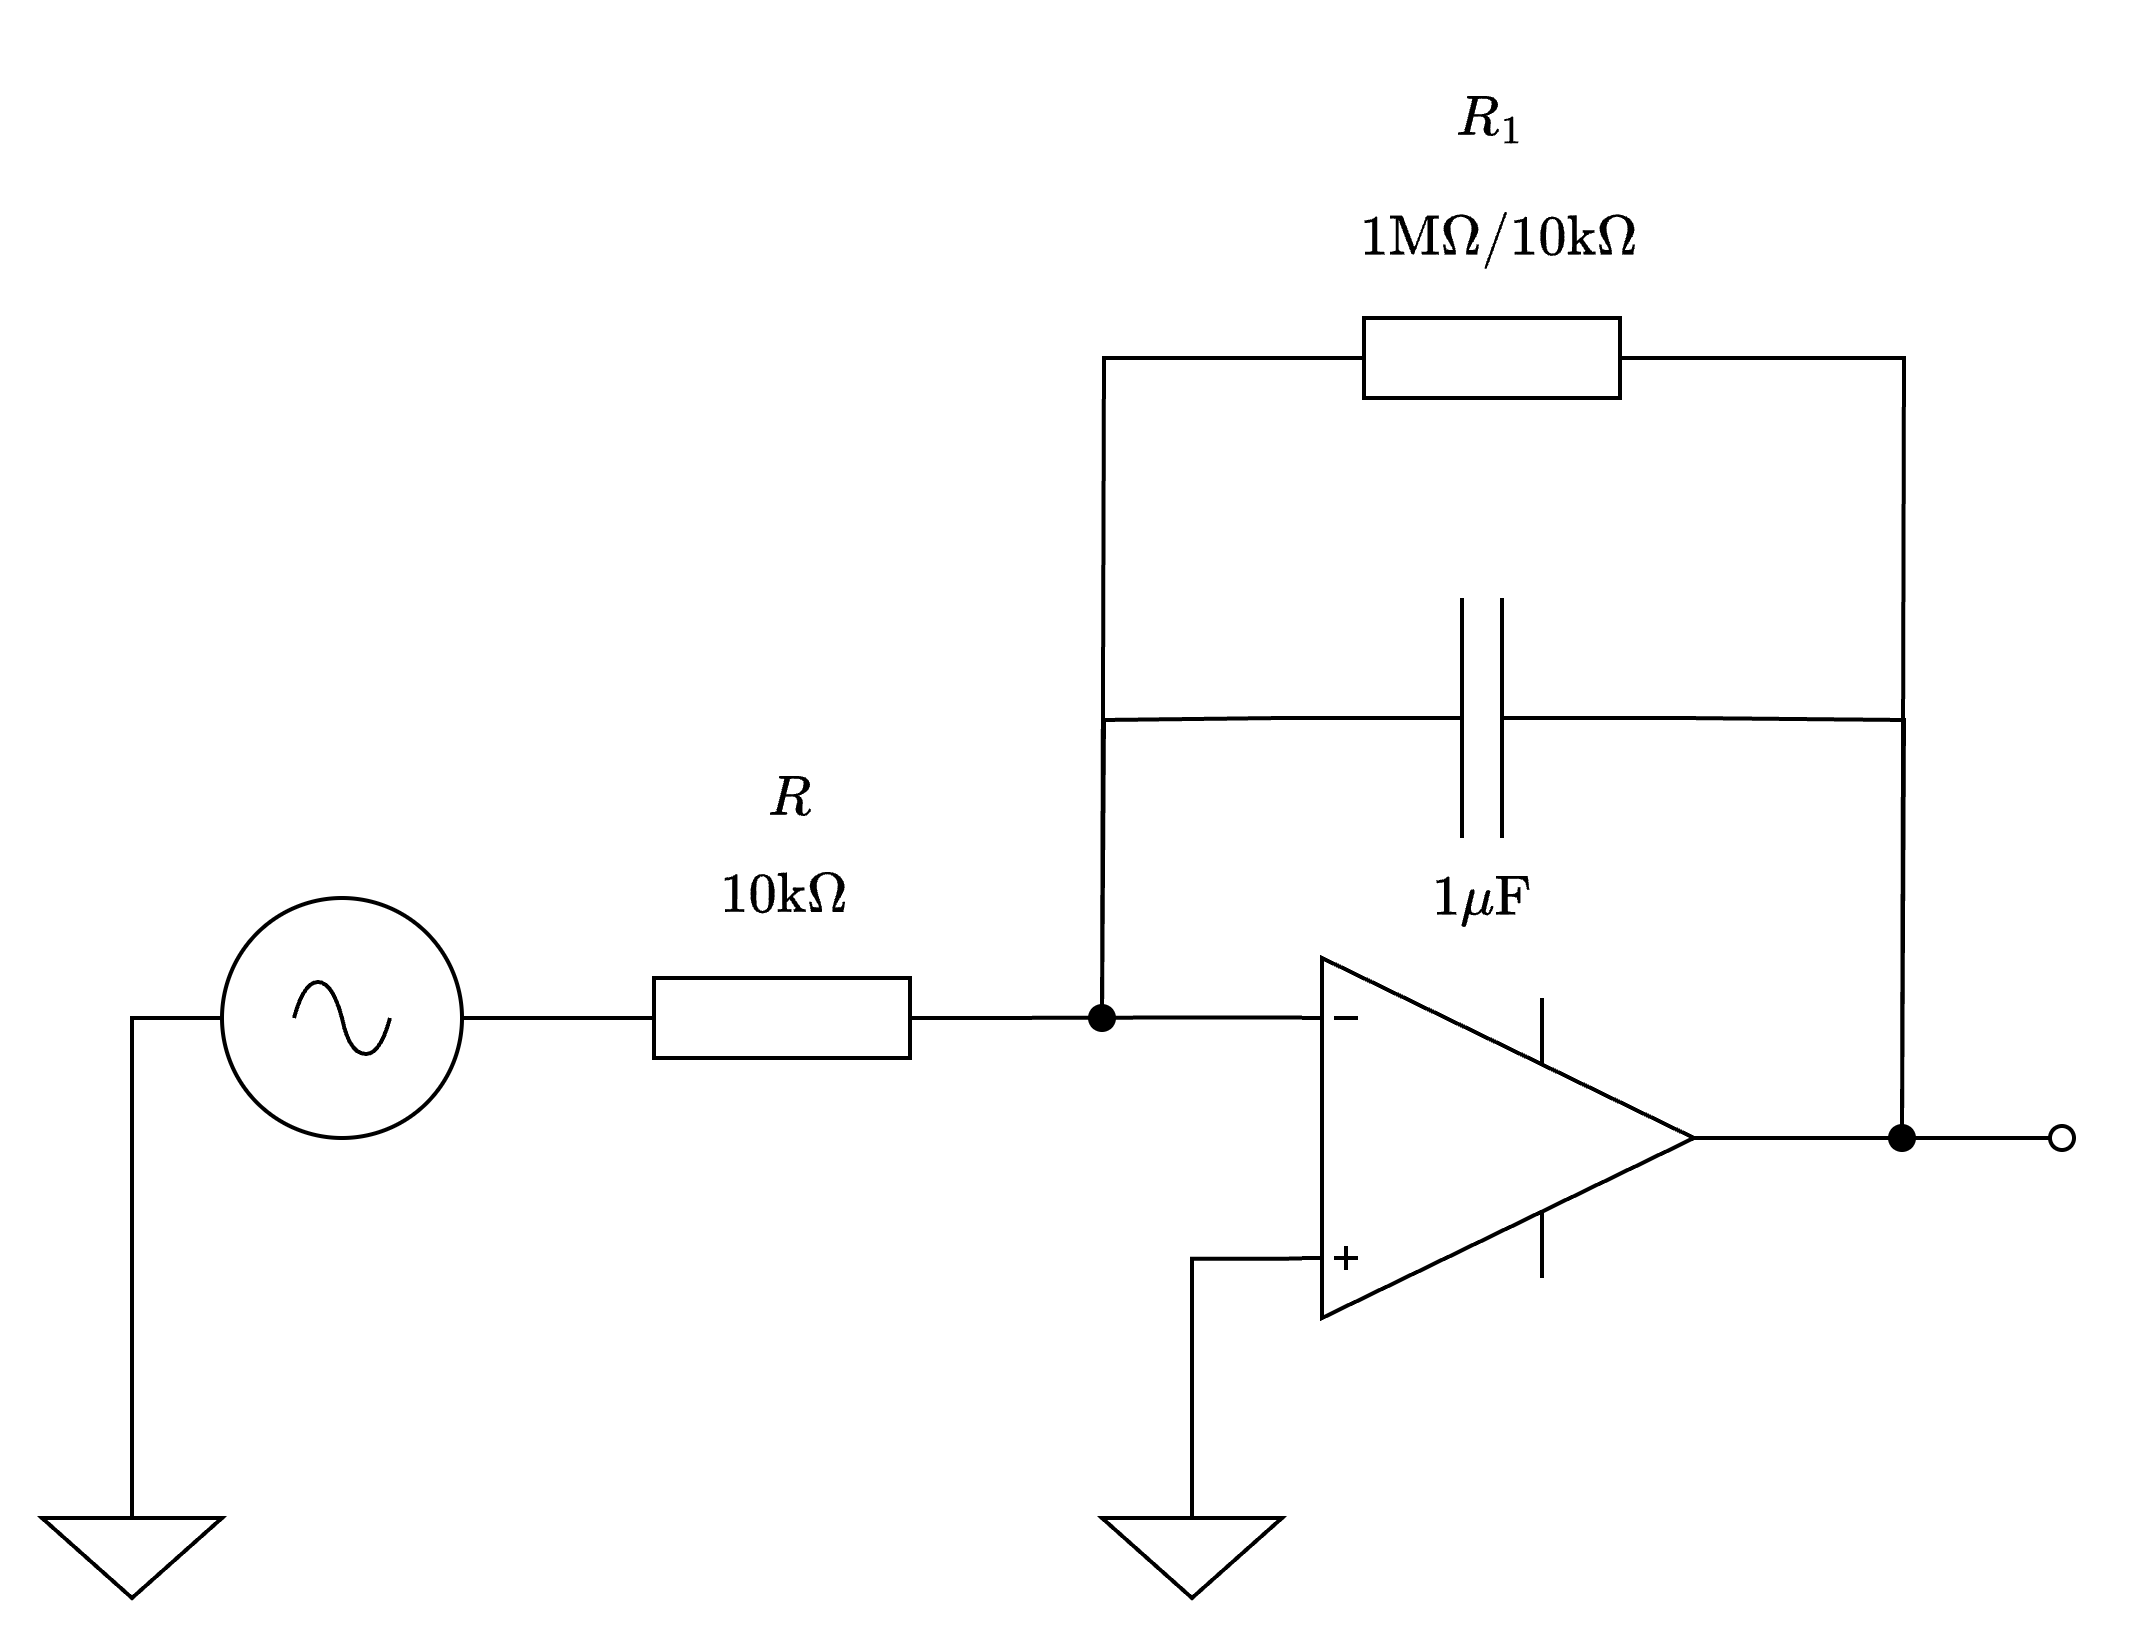
\includegraphics[width=0.8\linewidth]{src/figures/exp8/circuit.png}
	\caption{実験8 回路図}\label{fig:exp8-circuit}
\end{figure}

この回路に対して、Function Generatorからさまざまな周波数の正弦波を入力し、出力波形をオシロスコープで観察した。
周波数が大きくなるにつれ出力波形の振幅が小さくなっていった。
振幅が$1/\sqrt{2}=0.707$倍になる周波数は\SI{170}{Hz}でありその時の波形を図\ref{fig:exp8-raw-cutoff}に示す。
Bode Analayzerを用いてこの回路に\SI{1}{Hz}から\SI{100}{kHz}までの周波数の正弦波を入力し、ボード線図を作成した。
$R_1=\SI{10}{k\ohm}$と\SI{1}{M\ohm}の場合で比較したものを図\ref{fig:exp8-bode}に示す。

\subsection{実験9}\label{subsec:exp9}
まず今まで使用してきたオペアンプとは異なるオペアンプ2を用いて、図\ref{fig:exp9-circuit}に示すようなローパスフィルターを作成した。
\ref{subsec:exp8}と同様にBode Analayzerを用いてこの回路に\SI{1}{Hz}から\SI{100}{kHz}までの周波数の正弦波を入力し、ボード線図を作成した。
その後上記の回路と\ref{subsec:exp8}での回路を繋げ、ローパスフィルターを継続接続した図\ref{fig:exp9-circuit2}の回路を作成した。
\begin{figure}[!htb]
	\centering
	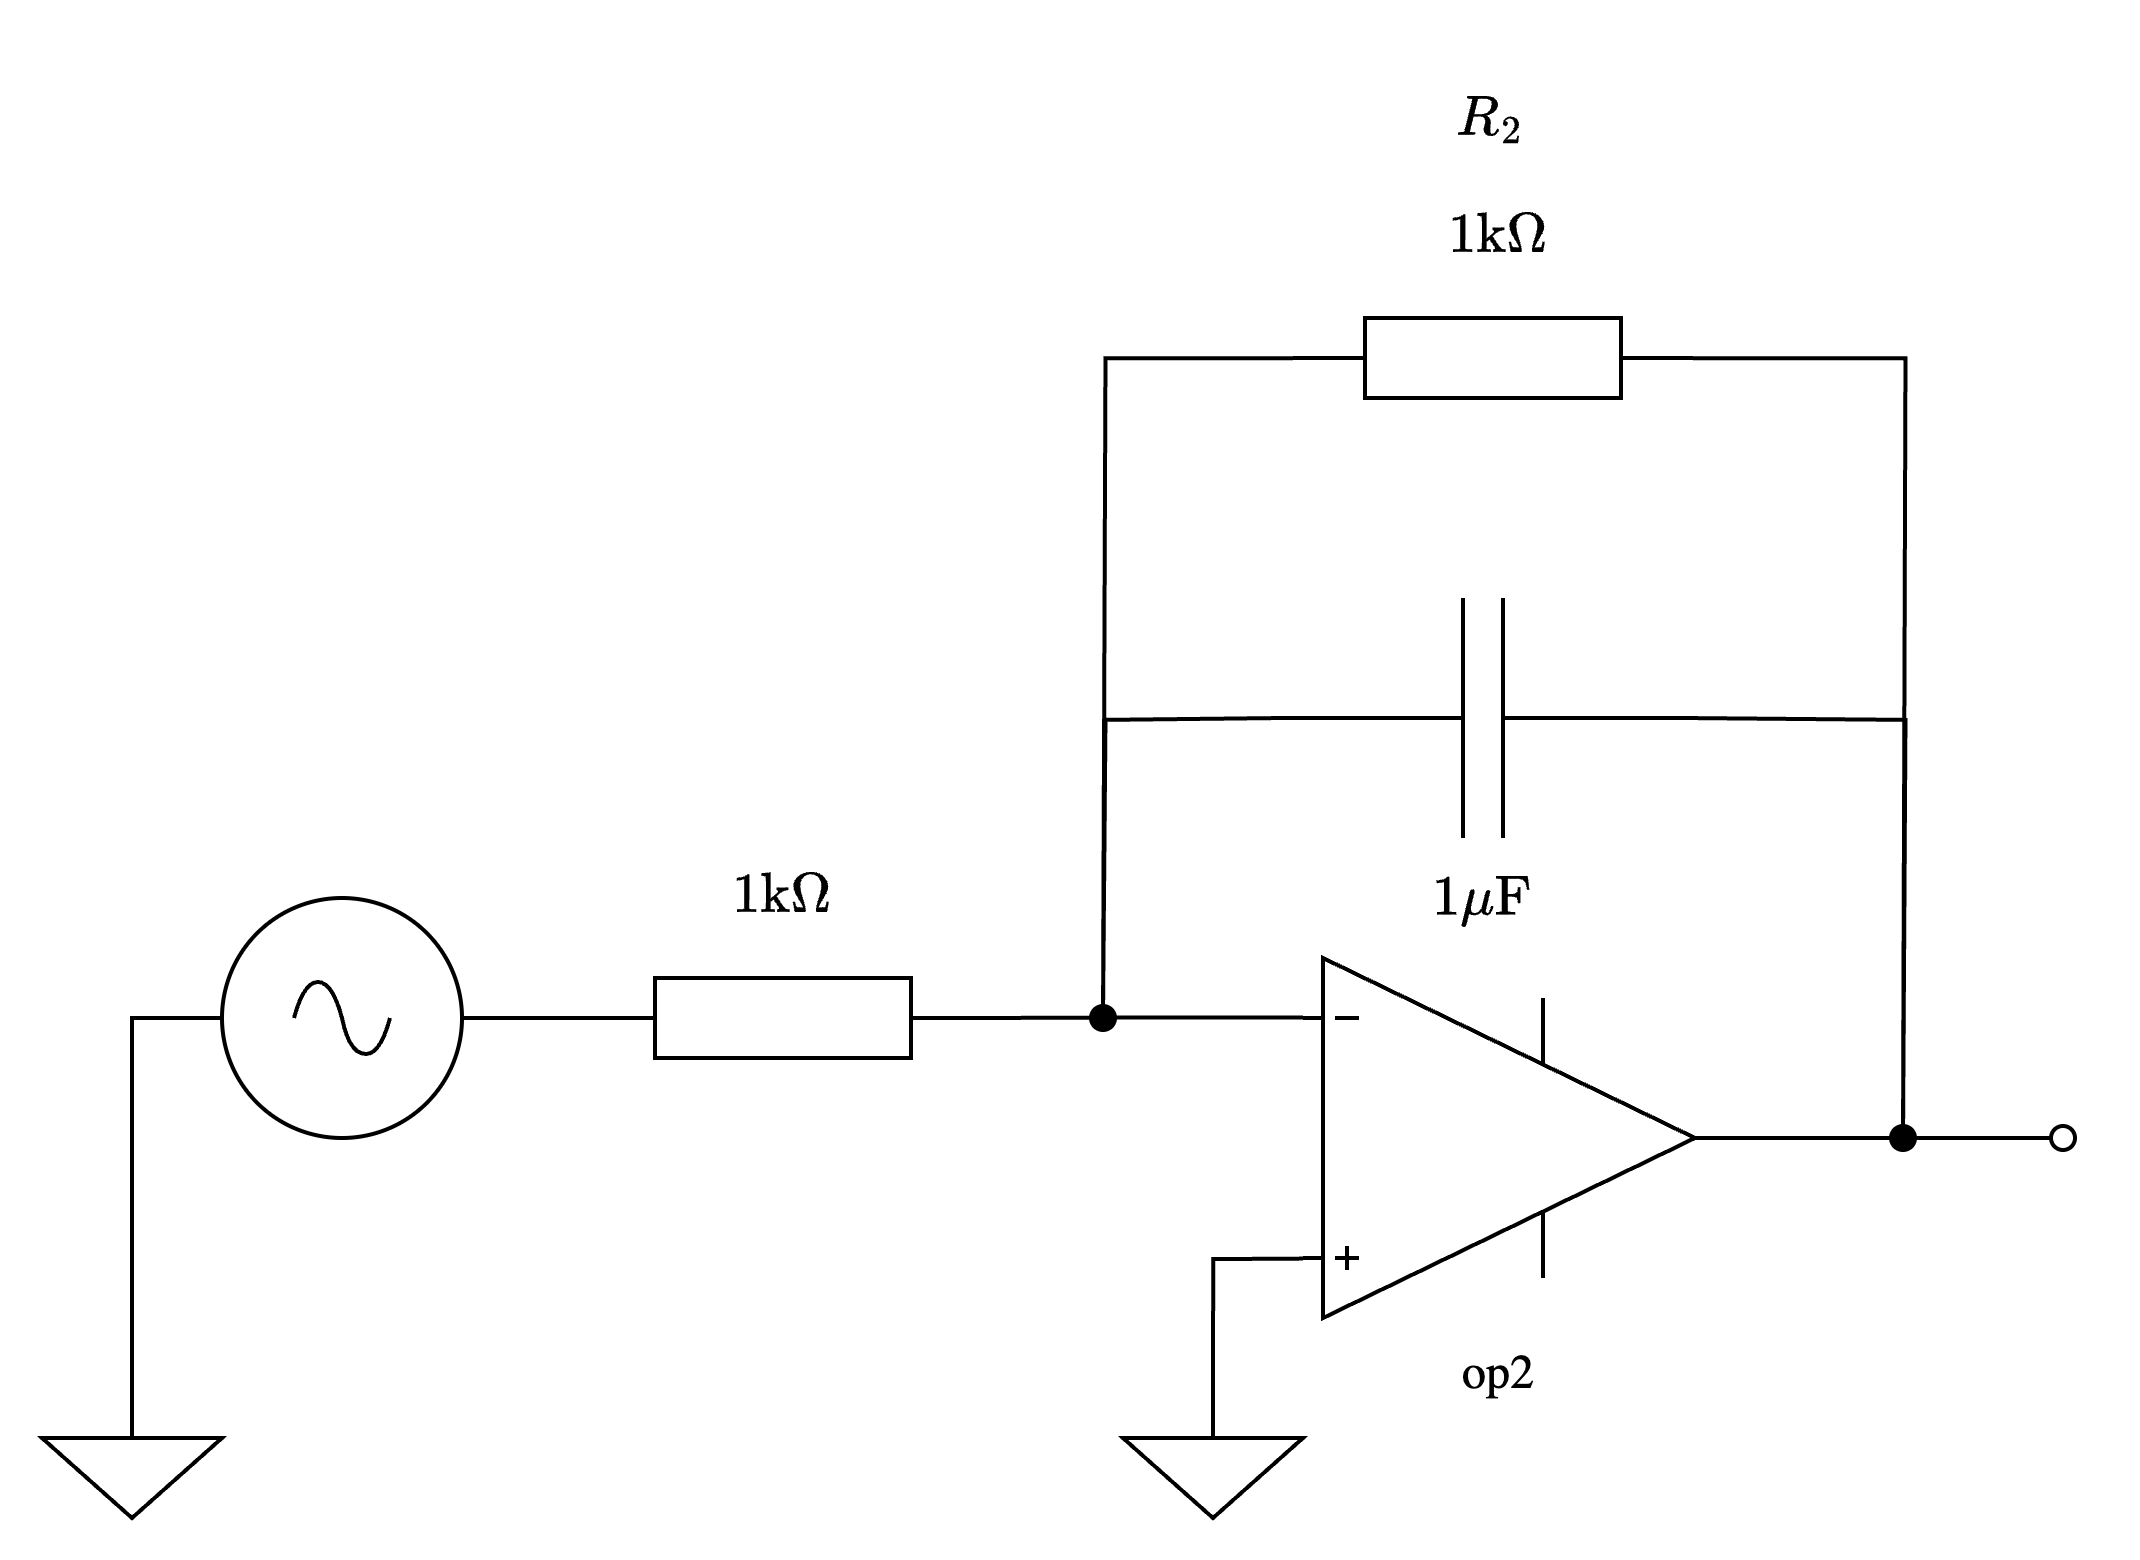
\includegraphics[width=0.9\linewidth]{src/figures/exp9/circuit.png}
	\caption{実験9 回路図}\label{fig:exp9-circuit}
\end{figure}

\begin{figure}[!htb]
	\centering
	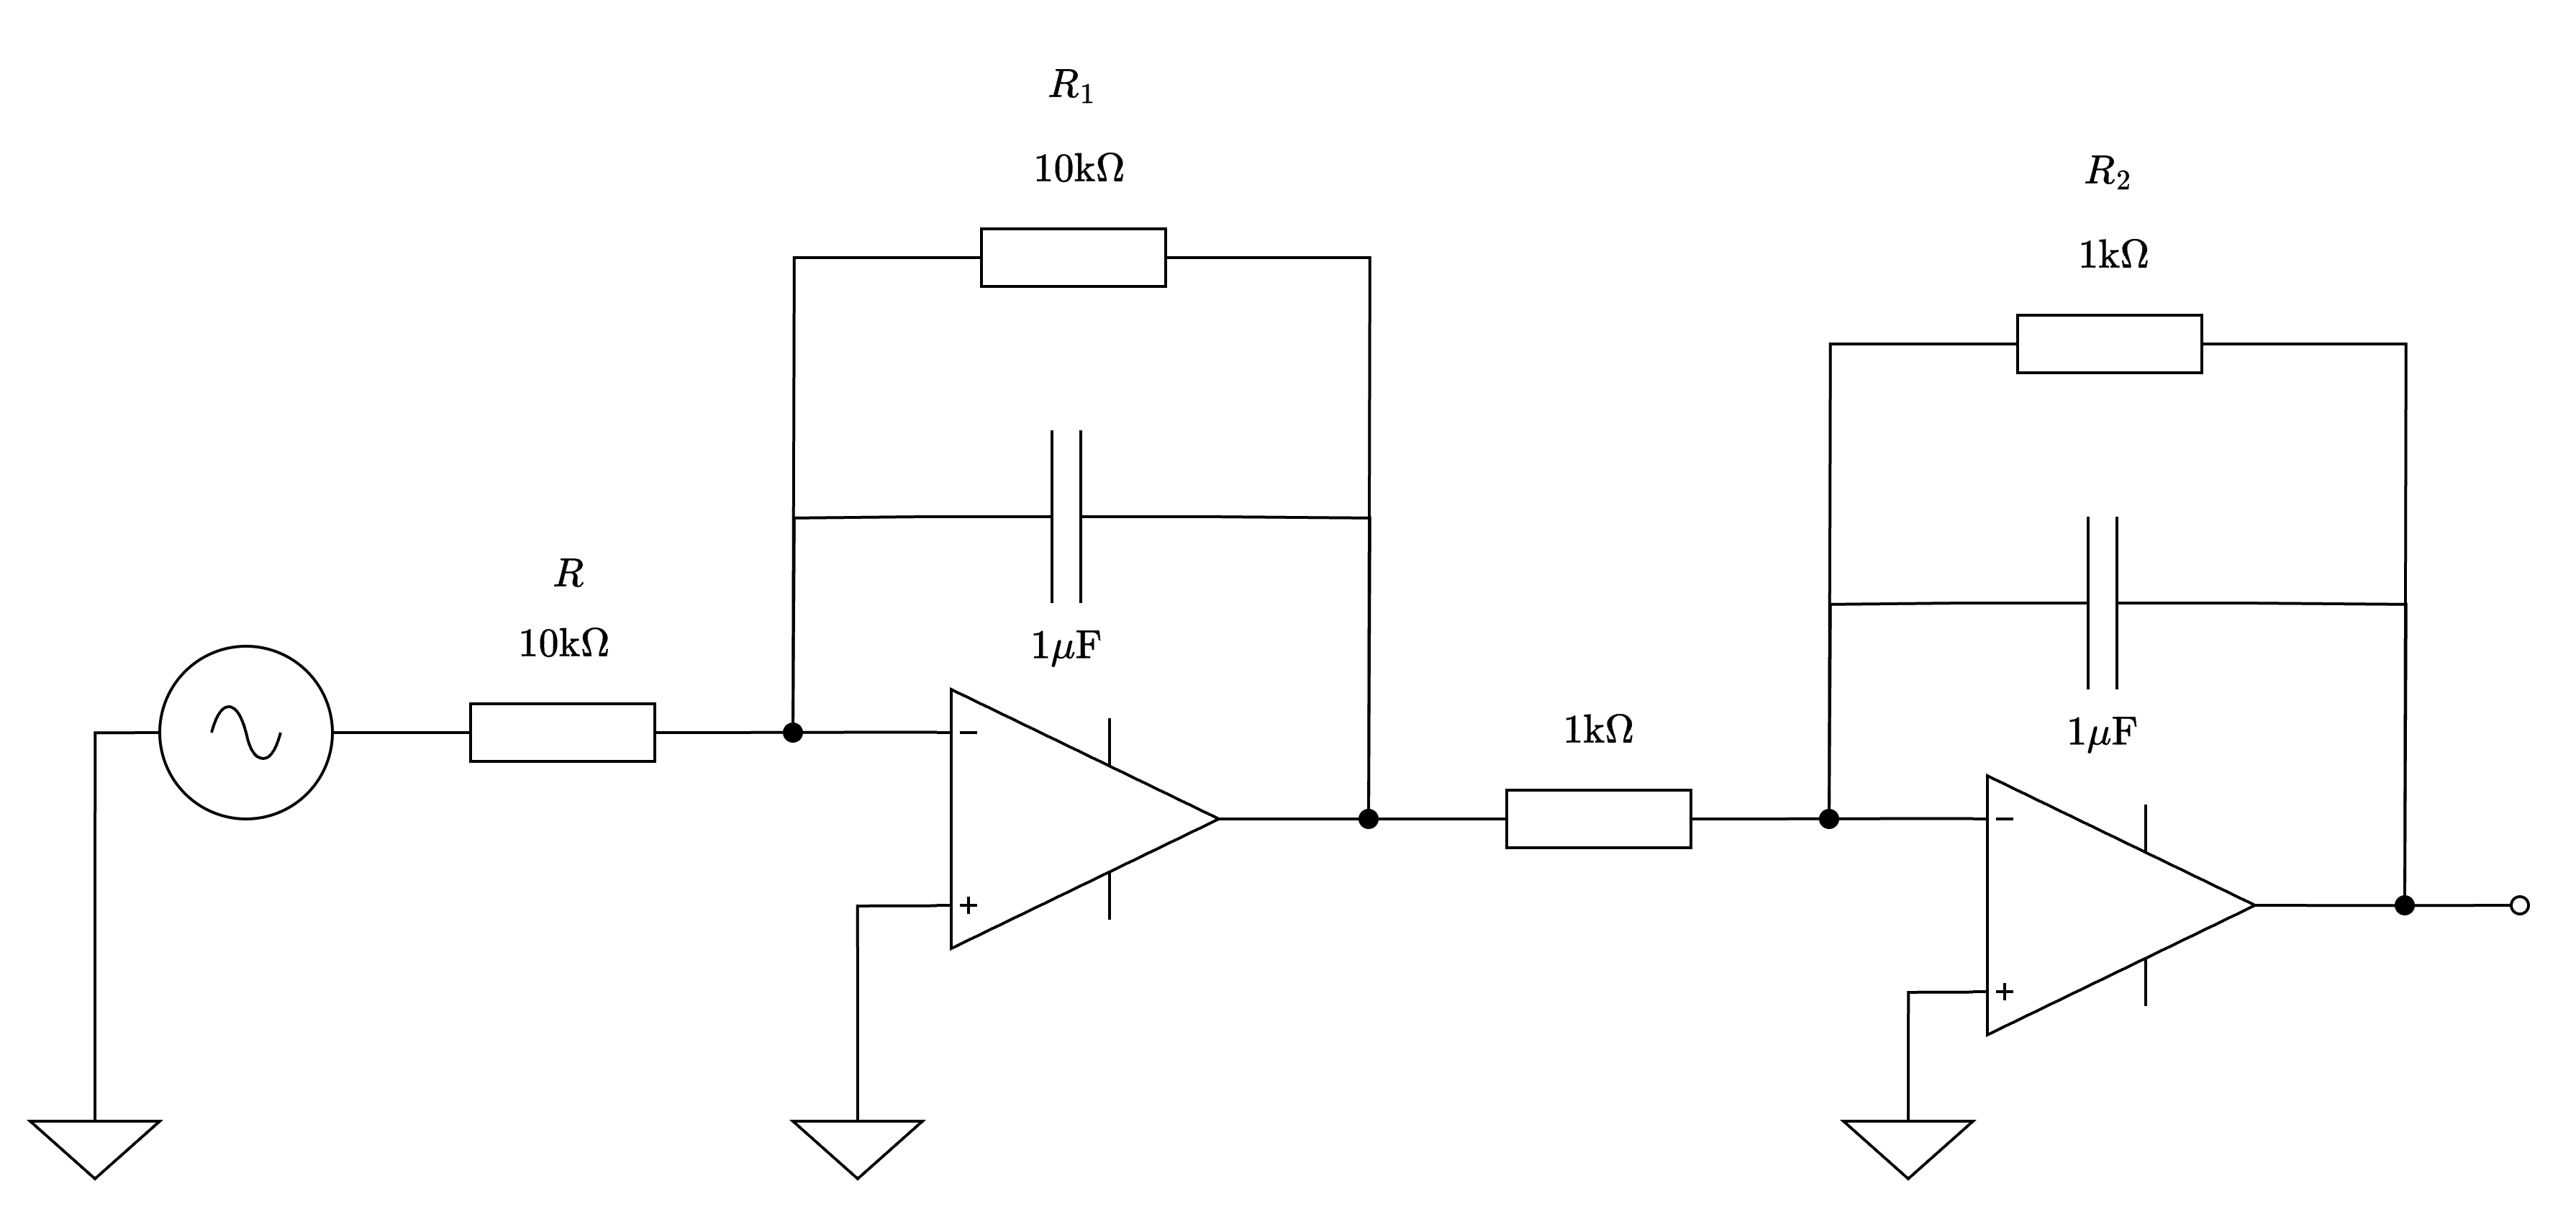
\includegraphics[width=0.9\linewidth]{src/figures/exp9/circuit2.png}
	\caption{実験9 回路図2}\label{fig:exp9-circuit2}
\end{figure}

それぞれの回路でのボード線図を図\ref{fig:exp9-bode}に示す。

\subsection{実験10}
\ref{subsec:exp9}の作成した回路から、図\ref{fig:exp10-circuit}に示すバイカット型フィルタを作成した。
\begin{figure}[!htb]
	\centering
	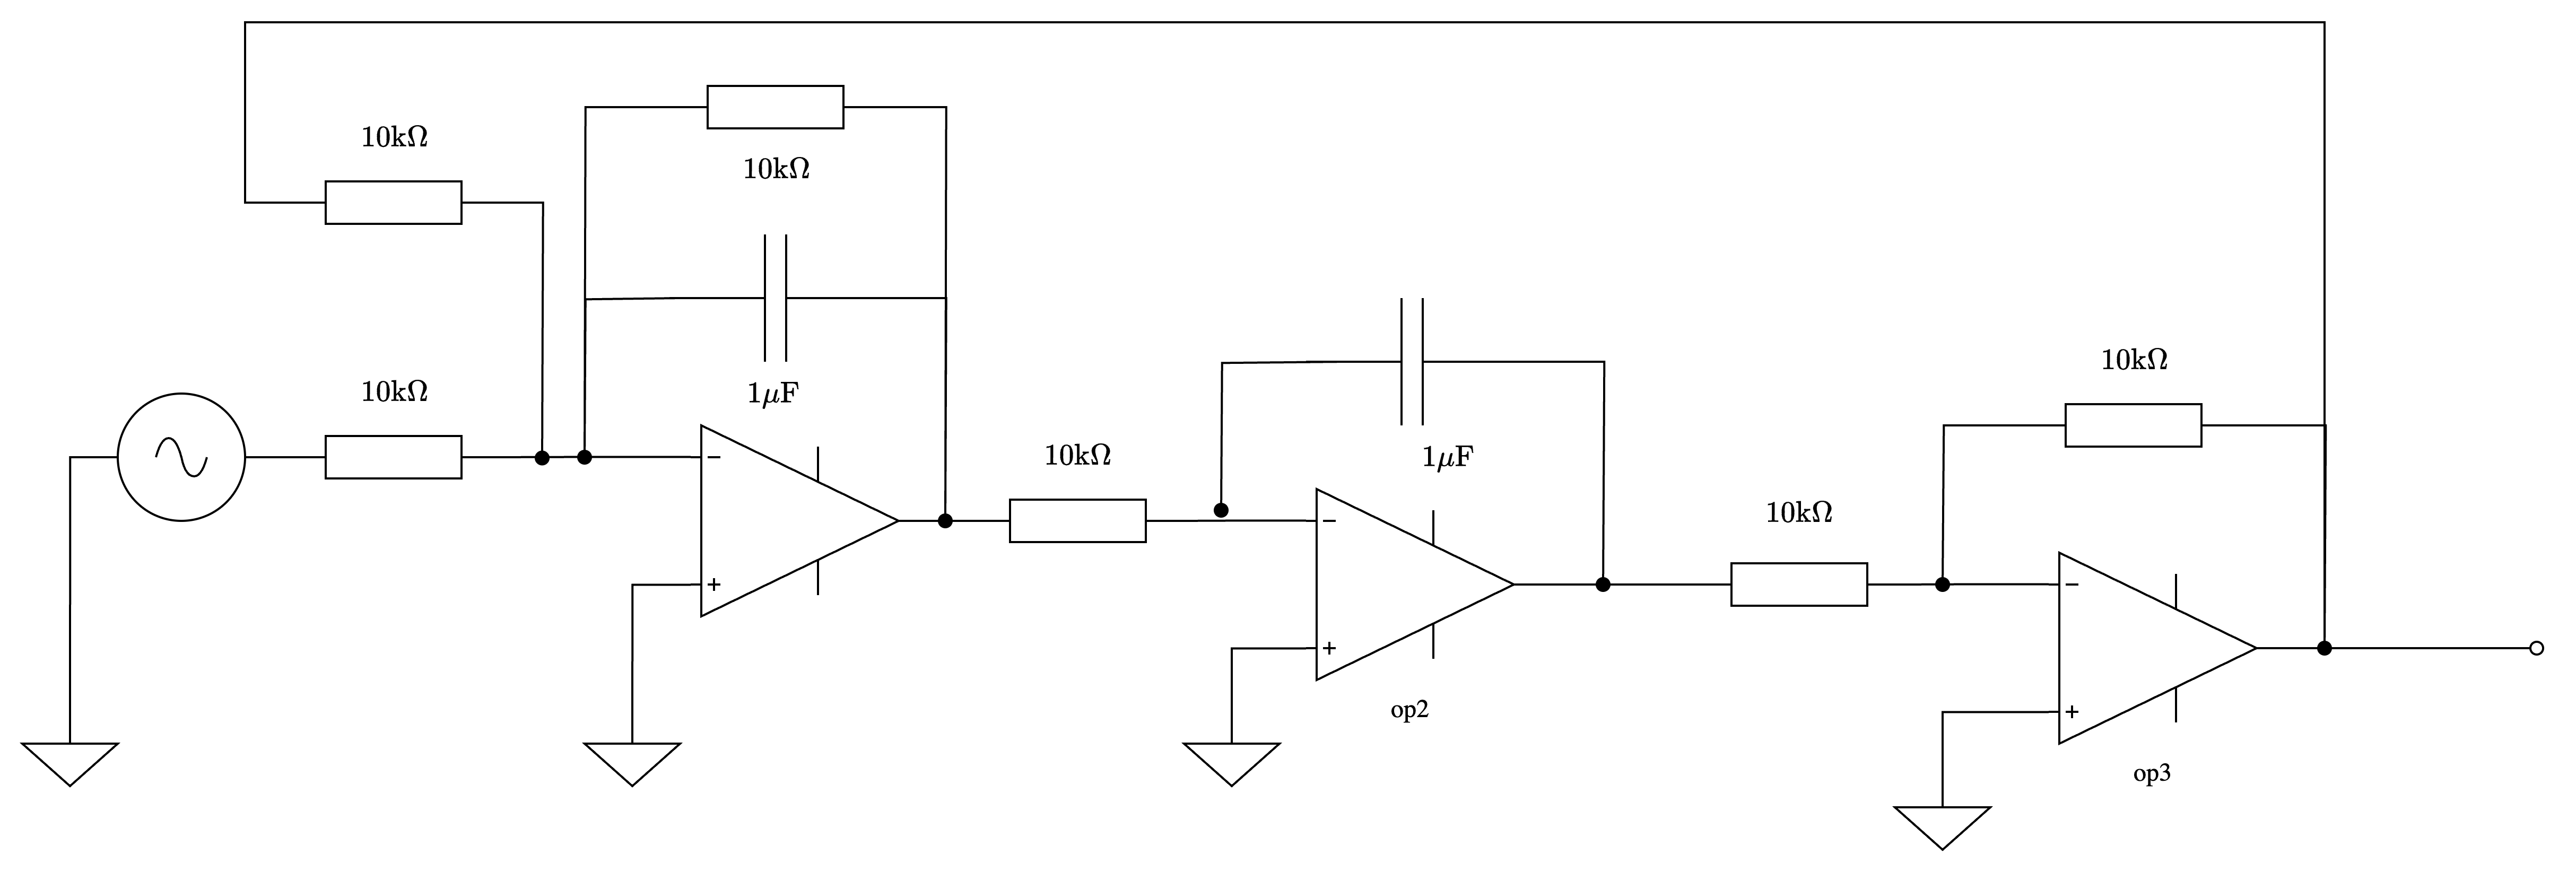
\includegraphics[width=0.90\linewidth]{src/figures/exp10/circuit.png}
	\caption{実験10 回路図}\label{fig:exp10-circuit}
\end{figure}

図中の$R_1$\SI{10}{k\ohm}でそれぞれ\SI{1}{Hz}から\SI{100}{kHz}までの周波数の正弦波を入力し
一番左のオペアンプの出力(反転ローパスフィルタの出力)と、一番右のオペアンプの出力(反転バンドパスフィルタの出力)の2つでボード線図を作成した。
その後、$R_1$を\SI{5}{k\ohm}、\SI{7}{k\ohm}、\SI{20}{k\ohm}のそれぞれで反転バンドパスフィルタの出力でボード線図を作成した。
撮影したボード線図の写真を図\ref{fig:exp10-bode}に示す。

次に反転バンドパスフィルタの出力にオシロスコープを繋げ、入力として矩形波を入力したときの波形を撮影した。
$R_1$を\SI{5}{k\ohm}、\SI{7}{k\ohm}、\SI{10}{k\ohm}、\SI{20}{k\ohm}のそれぞれで撮影した。
この撮影した写真を図\ref{fig:exp10-band-sq}に示す。
次に$R_1=\SI{20}{k\ohm}$として正弦波を入力し、\SI{20}{Hz}から\SI{180}{Hz}まで\SI{40}{Hz}刻みで変化させたときの出力波形を撮影した。
この撮影した写真を図\ref{fig:exp10-sin}に示す。




\end{document}
